\documentclass[12pt]{amsart}

% PACKAGES ~~~~~~~~~~~~~~~~~~~

\usepackage{amsfonts, amsthm, amssymb, amsmath, stmaryrd, etoolbox, mathtools}
\usepackage[margin=1in]{geometry}
\usepackage{graphicx,caption,subcaption}
\usepackage{tikz}
\usetikzlibrary{matrix,arrows}

% NEW COMMANDS ~~~~~~~~~~~~~~~

% common math shorthands
\newcommand{\RR}{\mathbb{R}}
\newcommand{\ZZ}{\mathbb{Z}}
\newcommand{\zmodtwo}{\ZZ / 2 \ZZ}
\newcommand{\rptwo}{\RR \mathbf{P}^2}
\newcommand{\NN}{\mathbb{N}}
\newcommand{\QQ}{\mathbb{Q}}
\newcommand{\CC}{\mathbb{C}}
\newcommand{\from}{\colon}
%\newcommand{\to}{\rightarrow}
%\newcommand{\gets}{\leftarrow}
\newcommand{\xto}[1]{\xrightarrow{#1}}
\newcommand{\xgets}[1]{\xleftarrow{#1}}
\newcommand{\inv}{^{-1}}
\newcommand{\bydef}{\coloneqq}

% fonts
\newcommand{\edit}[1]{{\color{red} #1 }}
\newcommand{\cat}[1]{\mathbf{#1}}
\newcommand{\type}[1]{\mathtt{#1}}

% types
\newcommand{\tin}{\colon}
\newcommand{\A}{\type{A}}
\newcommand{\B}{\type{B}}
\newcommand{\C}{\type{C}}
\renewcommand{\P}{\type{P}}
\newcommand{\Q}{\type{Q}}
\newcommand{\BAC}{\B +_{\A} \C}
\newcommand{\Type}{\type{Type}}
\newcommand{\ap}{\type{ap}}
\newcommand{\inl}{\type{inl}}
\newcommand{\inr}{\type{inr}}
\newcommand{\glue}{\type{glue}}
\newcommand{\refl}{\type{refl}}
\newcommand{\code}{\type{code}}
\newcommand{\encode}{\type{encode}}
\newcommand{\decode}{\type{decode}}

% math operators
\DeclareMathOperator{\Hom}{Hom}
\DeclareMathOperator{\id}{id}
\DeclareMathOperator{\ob}{Ob}
\DeclareMathOperator{\arr}{arr}
\DeclareMathOperator{\im}{im}
\DeclareMathOperator{\Aut}{Aut}
\DeclareMathOperator{\Bij}{Bij}
\DeclareMathOperator{\Sub}{Sub}

% theorem styles
\newtheorem{lemma}{Lemma}
\newtheorem{thm}{Theorem}
\newtheorem{prop}{Proposition}
\newtheorem{cor}{Corollary}
\theoremstyle{remark}
\newtheorem{rmk}{Remark}
\theoremstyle{definition}
\newtheorem{defn}{Definition}
\newtheorem{ex}{Example}

%%%%%%%%%%%%%
% begin document
%%%%%%%%%%%%%

\begin{document}
	
\title{Notes on a pushout of sets}
\maketitle

% ~~~~~~~~~~~~~~~~~~~~~~~~~~~~~~~~~
% ~~~~~~~~~~~~~~~~~~~~~~~~~~~~~~~~~
% ~~~~~~~~~~~~~~~~~~~~~~~~~~~~~~~~~
% ~~~~~~~~~~~~~~~~~~~~~~~~~~~~~~~~~

\section{HoTT concepts}

\begin{defn} \label{def:set}
  A \textbf{set} is a type $ \type{S} $
  such that for any elements $ x,y \tin \type{S} $, and
  $ p,q \tin x = y $, we have $ p = q $.
\end{defn}

\begin{defn} \label{def:ap}
  Let $ f \from \A \to \B $.  For any
  $ x,y \tin \A $, we get a function
  \[
    \ap_f \from x =_\A y \to fx =_\B fy
  \]
  On Identity types.
	
  This can be interpreted in three ways:
  \begin{enumerate}
  \item type morphisms preserve equality,
  \item functions of spaces are continuous,
  \item groupoid morphisms given functions on hom-sets.
  \end{enumerate}
  Because $ \ap $ preserve paths, all functions in HoTT are
  continuous.  There are more results showing that $ f $ is functorial
  in that it preserves refl's and path concatenation.
	
  \emph{Note: we can take the categorical notation and write
    $ f ( p ) $ for a path $ p \tin x = y $ instead of
    $ \ap_f ( p ) $, but for now we stick with the latter.}
\end{defn}

\begin{defn} % def : higher induction
	Types can be defined by constructors.
	For example the circle type $ \type{S}^1 $
	is given by a $ 0 $-cell $s$ and 
	a $ 2 $-cell $ p \tin s = s $.
	
	Higher induction says that to define
	a map out of such a type, it suffices
	to define the map on the constructors.
	Hence a map 
	\[
		f \from \type{ S }^1 \to \A
	\] 
	is given by $ f ( s ) $ and 
	$\ap_f ( p )$.
\end{defn}

\begin{defn} % def : pushout
\label{def:pushout}
	Given a span
	\[
	\begin{tikzpicture}
		\node (A) at (0,0) {$\A$};
		\node (B) at (1,0) {$\B$};
		\node (C) at (0,-1) {$\C$};
		\draw [->] (A) to 
			node [above] {\scriptsize $ f $} 
			(B);
		\draw [->] (A) to 
			node [left] {\scriptsize $ g $} 
			(C);
	\end{tikzpicture}
	\]
	its pushout $ \BAC $ is defined by
	\begin{itemize}
		\item a function 
			$ \inl \from \B \to \BAC $
		\item a function 
			$ \inr \from \C \to \BAC $
		\item for each $ a \in \A $ and path
			$ \glue ( a ) \tin fa = ga $
	\end{itemize}
	Hence, all functions $F \from \BAC \to \type{D}$
	are given by higher induction:
	\begin{itemize}
		\item define $ F ( \inl (b) ) $
			for all $ b \tin \B $
		\item define $ F ( \inr (c) ) $
			for all $ c \tin \C $
		\item define 
			$ \ap_{ F } ( \glue ( a ) ) \tin 
			 F ( \inl (fa) ) = F ( \inr (ga) ) $
			for all $ a \tin \A $
	\end{itemize}
\end{defn}

\pagebreak

% ~~~~~~~~~~~~~~~~~~~~~~~~~~~~~~~~~
% ~~~~~~~~~~~~~~~~~~~~~~~~~~~~~~~~~
% ~~~~~~~~~~~~~~~~~~~~~~~~~~~~~~~~~
% ~~~~~~~~~~~~~~~~~~~~~~~~~~~~~~~~~
% ~~~~~~~~~~~~~~~~~~~~~~~~~~~~~~~~~
% ~~~~~~~~~~~~~~~~~~~~~~~~~~~~~~~~~

\section{the setup}

The idea is that we have types 
$\A$, $\B$, and $\C$, all of which are sets. 
The question: is the pushout given by the square
\[ % pushoutsquare
  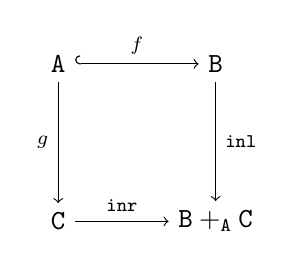
\begin{tikzpicture}
    \node (C) at (0,0) {$\C$};
    \node (BAC) at (2,0) {$\BAC$};
    \node (A) at (0,2) {$\A$};
    \node (B) at (2,2) {$\B$};
    \draw[right hook ->] (A) to node [above] {\scriptsize $f$} (B);
    \draw[->] (A) to node [left] {\scriptsize $g$} (C);
    \draw[->] (B) to node [right] {\scriptsize $\inl$} (BAC);
    \draw[->] (C) to node [above] {\scriptsize $\inr$} (BAC);
  \end{tikzpicture}
\]
also a set when $f$ is a monomorphism?

Thus to determine whether $\BAC$ is a set,
we need to access its identity types.  
We do this with an \emph{encode-decode} style proof.  

Roughly, a proof of this sort begins by guessing
what the identity types are.  That is,
for each $x$ and $y$ in $\BAC$, 
we define a type 
\[
	\code \from \BAC \to \BAC\to \Type
\]
so that $\code (x,y)$ serves as our guess  
as to what $x =_{\scriptsize \BAC} y$ actually is.  
Then we define functions
\[
	\type{ encode }_{ x , y } \from  ( x = y ) \to \code ( x , y ) 
	\text{ and }
	\type{ decode }_{ x , y } \from \code ( x , y ) \to ( x = y )
\]
for each $x$ and $y$ in $\BAC$.  
Hopefully, these are mutually inverse.

\pagebreak

% ~~~~~~~~~~~~~~~~~~~~~~~~~~~~~~~~~
% ~~~~~~~~~~~~~~~~~~~~~~~~~~~~~~~~~
% ~~~~~~~~~~~~~~~~~~~~~~~~~~~~~~~~~
% ~~~~~~~~~~~~~~~~~~~~~~~~~~~~~~~~~
% ~~~~~~~~~~~~~~~~~~~~~~~~~~~~~~~~~

\section{defining $\code$}

Let's try to define 
\[
	\code \from 
	\BAC \to \BAC \to \Type.
\]  
Note that $\code$ is a map from a pushout, 
so we define it using induction of higher types, 
as in Definition \ref{def:pushout}.
Hence we need three types schemes:
\begin{align*}
	\code(\inl(b)) & \from \BAC \to \Type \\
	\code(\inr(c)) & \from \BAC \to \Type \\
	\code( \ap_{\glue} (a) ) & \from \BAC \to \Type \\
\end{align*}
These schemes run through 
$a \tin A$, $b \tin B$, and $c \tin C$.  
They are also functions on the same coproduct!
To define $\code(\inl(b))$, 
we use higher induction which gives the type schemes:
\[
	\code(\inl(b),\inl(b')), \hspace{0.5em}
	\code(\inl(b),\inr(c')), \hspace{0.5em}
	\code(\inl(b),\ap_{\glue}(a')).
\]
Similarly, we define $\code(\inr(c))$ by
\[
	\code(\inr(c),\inl(b')), \hspace{0.5em}
	\code(\inr(c),\inr(c')) , \hspace{0.5em}
	\code(\inr(c),\ap_{\glue}(a')).
\]
and $\code(\glue(a))$ by 
\[
	\code(\ap_{\glue}(a),\inl(b')), \hspace{0.5em}
	\code(\ap_{\glue}(a),\inr(c')) , \hspace{0.5em} 
	\code(\ap_{\glue}(a),\ap_{\glue}(a')).
\]
The $\code$'s that have no $\ap_{\glue}$'s in the arguments correspond
to our guesses for the identity types.  The $\code$'s that have one
$\ap_{\glue}$ in the arguments give a pre- or post-composition of
paths.  The $\code$'s that have two $\ap_{\glue}$'s in the arguments
ensure that this pre- and post-composition action is coherent.  This
fits together in a nice little diagram:
\[ % coherence diagram for code
	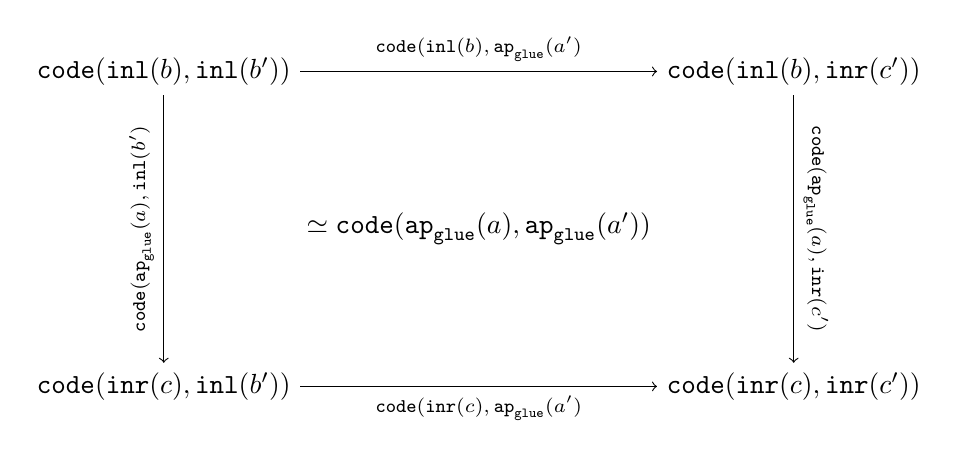
\begin{tikzpicture}
		\node (AA) at (0,0) 
			{ $ \simeq \type{ code } ( \ap_{\glue} ( a ) , \ap_{\glue} ( a' )  )$ }; 
		\node (BB) at (-4,2) 
			{ $ \type{ code } ( \inl( b ) , \inl( b' )  )$ }; 
		\node (BC) at (4,2) 
			{ $ \type{ code } ( \inl( b ) , \inr( c' )  )$ }; 
		\node (CB) at (-4,-2) 
			{ $ \type{ code } ( \inr( c ) , \inl( b' )  )$ }; 
		\node (CC) at (4,-2) 
			{ $ \type{ code } ( \inr( c ) , \inr( c' )  )$ }; 
		\draw [->] (BB) to 
			node 
				[above] 
				{\scriptsize $ \type{ code } ( \inl( b ) , \ap_{\glue} ( a' ) $ } 
			(BC);
		\draw [->] (BB) to 	
			node 
				[rotate=90,above] 
				{ \scriptsize $ \type{ code } ( \ap_{\glue} ( a ) , \inl( b' ) $ } 
			(CB);
		\draw [->] (BC) to 
			node 
				[rotate=-90, above] 
				{\scriptsize $\type{ code } ( \ap_{\glue} ( a ) , \inr( c' ) $} 
			(CC);
		\draw [->] (CB) to 	
			node 
				[below] 
				{ \scriptsize $ \type{ code } ( \inr( c ) , \ap_{\glue} ( a' ) $ } 
			(CC);
	\end{tikzpicture}
\]

%%%%%%%%%%%%%%%%%
\pagebreak
\subsection*{code( b,b')}

$\code \left( \inl ( b ) , \inl( b' ) \right)$ is the most complicated. 
In order to incorporate $\type{ refl }_b$ when $b$ is not in the image of $f$, 
we define this type to be the pushout of the span
\[
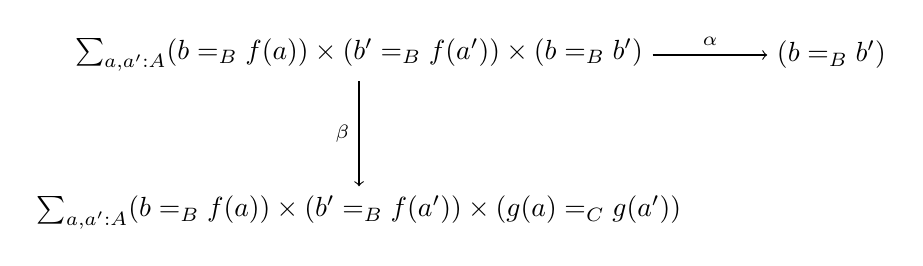
\begin{tikzpicture}
	\node (1) at (0,2) 
		{ $ \sum_{ a , a' : A } 
			( b =_B f ( a ) ) 
			\times ( b' =_B f ( a' ) ) 
			\times ( b =_B b' ) $ };
	\node (2) at (6,2) 
		{ $ ( b =_B b' ) $ };
	\node (3) at (0,0) 
		{ $ \sum_{ a , a' : A } 
			( b =_B f ( a ) ) 
			\times  (b' =_B f ( a' ) ) 
			\times ( g ( a ) =_C g ( a' ) ) $ };
	\draw [ -> ] (1) to 
		node [above] {\scriptsize $ \alpha $} 
		(2);
	\draw [ -> ] (1) to 
		node [left] {\scriptsize $ \beta $}
		(3);
\end{tikzpicture}
\]
Here, $ \alpha $ is a projection. Also,
$ \beta $ is a projection of the first
two factors and places $ \type{ ap }_g (p) $ 
in the third factor. This uses the injectivity of $f$
to get a $ p \tin a = a' $ if the upper left
is populated.

This is a proposition. 
Indeed, the span feet are propositions
and the only way for both to be populated
is if the apex is also populated.
But this would identify the 
left and right included elements
with a glue.

But this can be simplified via some case analysis. If $ (p,q,r) $ is
in the upper left, then since we know that we get a path
$ q r p^{-1} : fa =_{\B} fa' $ which gives a $ \ell : a =_{\A} a' $ by
injectivity of $ f $.  Thus we can $ \beta $-reduce $ fa' $ to $ fa $
which gives us
$ (b=_{\B} fa) \times (b'=_{\B} fa) \times (b=_{\B} b') $.  Any
witness to that has form $ (p,q',r) $ where $ q^{-1}p : b =_{\B} b' $
so since $ \B $ is a set, $ q^{-1}p = r $ so this
$ (p,q',r) = (p,q',q^{-1}p) $.  Since the last factor depends on the
first two, we can ignore it so we reduce the upper left further to
$ (b=_{\B} fa) \times (b'=_{\B} fa) $.  But maybe a nicer thing to
work with is
$ (b=_{\B} fa) \times (b'=_{\B} fa') \times (a =_{\A} a') $.  Then
$ \alpha $ assembles those maps into one of form $ b =_{\B} b' $ and
$ \beta $ applies $ g $ to the last factor. That is, we can work
instead with the pushout
\[
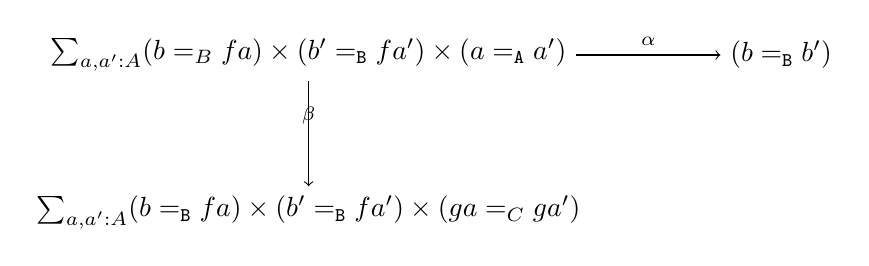
\begin{tikzpicture}
	\node (1) at (0,2) 
	{ $ \sum_{ a , a' : A } 
		( b =_B f  a ) 
		\times ( b' =_{\B} f  a' ) 
		\times ( a =_{\A} a' ) $ };
	\node (2) at (6,2) 
	{ $ ( b =_{\B} b' ) $ };
	\node (3) at (0,0) 
	{ $ \sum_{ a , a' : A } 
		( b =_{\B} f a ) 
		\times  (b' =_{\B} f a' ) 
		\times ( g a =_C g a' ) $ };
	\draw [ -> ] (1) to 
	node [above] {\scriptsize $ \alpha $} 
	(2);
	\draw [ -> ] (1) to 
	node [above] {\scriptsize $ \beta $}
	(3);
\end{tikzpicture}
\]
We can simplify this further due to the injectivity of $ f $.  The apex of the span can be boiled down to  
\[
	( b =_{\B} fa ) \times ( b' =_{\B} fa' ) \times ( a =_{\A} a' )  
\] 
is equivalent to 
\[
	( b =_{\B} fa ) \times ( b' =_{\B} fa ) 
\]
because if all three factors are populated, then we can $ \beta $-reduce $ a' $ to $ a $ and $ a =_{\A} a $ contains only $ \refl $ because $ \A $ is a set.  Thus, our pushout becomes
\[
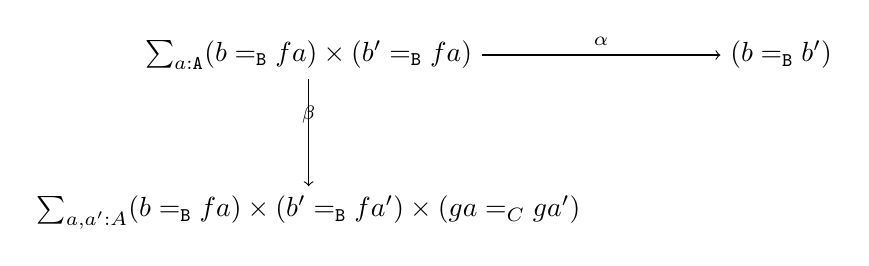
\begin{tikzpicture}
	\node (1) at (0,2) 
		{ $ \sum_{ a : \A } 
		( b =_\B f  a ) 
		\times ( b' =_{\B} f  a ) $} ; 
	\node (2) at (6,2) 
		{ $ ( b =_{\B} b' ) $ };
	\node (3) at (0,0) 
		{ $ \sum_{ a , a' : A } 
		( b =_{\B} f a ) 
		\times  (b' =_{\B} f a' ) 
		\times ( g a =_C g a' ) $ };
	\draw [ -> ] (1) to 
		node [above] {\scriptsize $ \alpha $} 
		(2);
	\draw [ -> ] (1) to 
		node [above] {\scriptsize $ \beta $}
		(3);
\end{tikzpicture}
\]


Later, when defining $ \decode $, we'll need to know what constructors this pushout has.  
\begin{itemize}
	\item $  \sum_{ a , a' : A } ( b =_B f  a ) \times ( b' =_{\B} f  a' ) \times ( a =_{\A} a' ) $.  Any witnesses $ (p,q,\ell) $ assembles into a path $ b =_{\B} b' $ so $ \alpha $ is injective.  Since $ \B $ is a set, this is a proposition.
	\item $  \sum_{ a , a' : A } ( b =_B f  a ) \times ( b' =_{\B} f  a' ) \times ( a =_{\A} a' ) $ .  This can only contain one element.  Indeed, suppose that $ (p,q,r) : ( b =_B f  a ) \times ( b' =_{\B} f  a' ) \times ( a =_{\A} a' ) $ and $ (p',q',r') : ( b =_B f  a'' ) \times ( b' =_{\B} f  a''' ) \times ( a'' =_{\A} a''' ) $ witness the lower left.  Then $ p $ and $ p' $ assemble to witness $ fa =_{\B} fa'' $. Similarly, $ q $ and $ q' $ assemble to witness $ fa' =_{\B} fa''' $. By injectivity of $ f $, we get than $ a =_{\A} a'' $ and $ a' =_{\A} a''' $.  So $ ( b =_B f  a'' ) \times ( b' =_{\B} f  a''' ) \times ( a'' =_{\A} a''' ) $ beta-reduces to $ ( b =_B f  a ) \times ( b' =_{\B} f  a'' ) \times ( a' =_{\A} a' ) $. This reduction identifies $ (p,q,r) $ and $ (p',q',r') $ because each factor is a set.  So the lower left is a proposition.
\end{itemize}

From this, it follows that both $ \alpha $ and $ \beta $are injections and so the pushout is a set by some older result (ask mike).  Anyway, depending on a few things we have different cases.
\begin{rmk} \label{rmk_code-bb-cases}
\begin{itemize}
	\item If $ p : b =_{\B} b' $ neither $ b,b' $ in the image of $ f $, then the only constructor of the pushout is $ \inl p $.
	\item If $ p : b =_{\B} b' $ and $ b $ is in the image of $ f $, then so is $ b' $.  Then the upper left is populated, which implies the lower left is and so the constructor are the elements included from the upper right and lower left which are then glued together.
	\item If $ b =_{\B} b' $ is empty is either $ b $ or $ b' $ are not in the image of $ f $ then both other corners are empty too, so no constructors.
	\item If $ b =_{\B} b' $ is empty, $ p: b =_{\B} fa $ and $ q : b' =_{\B} fa' $, then $ a =_{\A} a' $ must be empty, else we can prove $ b=_{\B}b' $. Hence upper right and upper left are empty.  So either $ ga =_{\C} ga' $ is empty or not.  If not, we get a constructor included from the lower left, else the pushout is empty.  
\end{itemize}
\end{rmk}

%
% commented out is discussion 
% to understand the pushout
%
%\begin{itemize}
%	\item Case 1---$ b,b' $ not in the image of $ f $, then only upper right can be non-empty, so $\type{ code } ( \inl( b ) , \inl( b' ) )$ is $ b =_{\B} b' $.
%	\item Case 2---$ b $ alone is in the image of $ f $. That is, for some $ a $, $ b =_{\B} fa $ is occupied, but for no $ a' $ is $ b=_{\B} fa' $ occupied.  It follows that $ b=_{\B} b' $ is empty, because otherwise $ b' =_{\B} b =_{\B} fa $.  Hence $\type{ code } ( \inl( b ) , \inl( b' ) )$ is empty.
%	\item Case3---$ b' $ alone is in the image of $ f $ mirrors case 2 by symmetry. Hence $\type{ code } ( \inl( b ) , \inl( b' ) )$ is empty.
%	\item Case 4---there exists $ a,a' : \A $ with $ b =_{\B} fa $ and $ b' =_{\B} fa' $.  There are two subcases here.
%	\begin{itemize}
%		\item Case 4a---$fa =_{\B} fa' $ is occupied. By injectivity of $ f $ we get $ \ell : a =_{\A} a' $ such that $ \ap_{f} \ell =_{\B} \ell $.  Given $ (p,q,r) $ in upper left, since $ \A $ is a set, we have that $ r =_{b =_{\B} b'} q^{-1}(\ap_{f}\ell) p $. Hence $ (p,q,r) =_{\text{upper left}} (p,q,q^{-1}(\ap_{f}\ell)p) $.  Now $ b=_{\B}b' $ is occupied and the witness must (since $ \B $ is a set) be $ \alpha (p,q,q^{-1}(\ap_{f}\ell) p) \coloneqq  q^{-1}\ell p$.  Moreover, $ \beta (p,q,q^{-1}(\ap_{f}\ell) p) \coloneqq = (p,q, \ap_{g} \ell) $. Hence this pushout has constructors $\inr (q^{-1}(\ap_{f}\ell)p) $, $ \inl (p,q, \ap_{g} \ell) $, and $ \glue (p,q,r) : \inr (q^{-1}(\ap_{f}\ell) p) = \inl (p,q, \ap_{g} \ell) $.  Are these all the constructors?  There are no more coming from $ b =_{\B} b' $ since $ \B $ is a set. To come from the bottom left, there must exist $ a'' , a''' : \A $ such that $ b =_{\B} fa'' $ and $ b' =_{\B} fa''' $. Then concatenating paths gives us $ fa =_{\B} fa'' $ and $ fa' =_{\B} fa''' $, which by injectivity of $ f $ means $ a =_{\A} a'' $ and $ a' =_{\A} a''' $. 
%		For this case, we assume that $ fa=_{\B}fa' $ is occupied, which now means that $ fa''=_{\B}fa''' $ and, by injectivity of $ f $, $ \ell' : a''=_{\A}a''' $.  Thus, in the lower left of the pushout square, there are two witnesses: $ (a,a',p,q,\ap_{f}\ell) $ and $ (a'',a''',p',q',\ap_{f}\ell') $. Now, since $ p' p^{-1} : fa =_{\B} fa'' $ and $ q' q^{-1} : fa' =_{\B} fa''' $, we get an $ \ell'' : a =_{\A} a'' $ and $ \ell''' : a' =_{\A} a''' $.  This gives $ \ell' \ell'' , \ell ''' \ell : a =_{\A} a''' $ which must commute because $ \A $ is a set.  Applying $ g $ to this square, we get a u
%		
%		{\color{red} are there any more elements being inl'ed from b=fa'' or b'=ba''' in this situation?}
%		\item Case 4b---$ fa =_{\B} fa' $ is not occupied
%	\end{itemize}
%\end{itemize}

%%%%%%%%%%%%%%%%%
\pagebreak
\subsection*{code (b,c)}

$
	\type{ code } \left( \inl( b ) , \inr( c' ) \right) \coloneqq
	\sum_{ a : A } ( b =_B f ( a ) ) \times ( c' =_C g ( a ) )
$
This is a proposition. 
Indeed, if there does not exist an $ a : A $ such that
$ b =_B f ( a )$ and $ c' =_C g ( a ) $
are both populated, then 
$ \type{ code } \left( \inl( b ) , \inr( c' ) \right) $ 
is empty. 
If there exists a single $a : A$ such that 
$ b =_B f ( a )$ and $ c' =_C g ( a ) $
are both populated, then 
because they are each equivalent to $ \type{ 1 }$,
$ \type{ code } \left( \inl( b ) , \inr( c' ) \right) $ 
is also equivalent to $ \type{ 1 }$.
If there is $a, a' : A$ such that
$ b =_B f ( a )$ and $ c' =_C g ( a ) $,
and also 
$ b =_B f ( a' )$ and $ c' =_C g ( a' ) $,
then the injectivity of $f$ and
$f ( a ) =_B b =_B f ( a' )$ 
implies that
$a =_A a'$
which also gives us that 
$ \type{ code } \left( \inl( b ) , \inr( c' ) \right) $ 
is equivalent to $ \type{ 1 }$.

%%%%%%%%%%%%%%%%%
\pagebreak
\subsection*{code (c,b)}

	$ \type{ code } \left( \inr( c ) , \inl( b' ) \right) \coloneqq \sum_{ a : A } ( c =_C g ( a ) ) \times ( b' =_B f ( a ) ) $
	This is a proposition by the same sort of argument from above.

%%%%%%%%%%%%%%%%%%
\pagebreak
\subsection*{code (c,c')}

	$ \type{ code } \left( \inr( c ) , \inr( c' ) \right) \coloneqq \sum_{ a , a' : A } ( c =_C g ( a ) ) \times ( c' =_C g ( a' ) ) \times ( f ( a ) =_B f ( a' ) ) $ 	
	The injectivity of $f$ gives us that 
	$ f ( a ) =_B f ( a' ) $
	imples that 
	$ a =_A a'$
	which in turn implies that
	$ g ( a ) =_C g ( a' )$,
	hence 
	$ c =_C c'$.
	Therefore, 
	$
	\type{ code } \left( \inr( c ) , \inr( c' ) \right) =	
	\left( c =_C c'  \right). 
	$
	Hence 
	$ \type{ code } \left( \inr( c ) , \inr( c' ) \right) $
	is a proposition.

%%%%%%%%%%%%%%%%%%%%
\pagebreak
\subsection*{code (b, glue a)}

These are all equivalences, hence by univalence
we define them as identity types. 
To show this, we show each is populated.

	$ 
	\type{ code } \left( \inl( b ) , \type{ ap }_{ \type{ glue } } ( a' ) \right) \colon \left( \type{ code } ( \inl( b ) , \inl( f ( a' ) ) ) = \type{ code } ( \inl( b ) , \inr( g ( a' ) ) ) \right) 
	$
	Because both sides of the identity type are propositions,
	to show that this equivalence holds
	it suffices to show that either
	$\type{ code } ( \inl( b ) , \inl( f ( a' ) ) )$
	and
	$\type{ code } ( \inl( b ) , \inr( g ( a' ) ) )$
	are both empty or both populated.
	This follows from post-composition with
	$ \type{ glue ( a' ) }$
	or its inverse.	

%%%%%%%%%%%%%%%%%%%%
\pagebreak
\subsection*{code (glue a, b)}

	$ 
	\type{ code } \left( \type{ ap }_{ \type{ glue } } ( a ) , \inl( b' ) \right) \colon
	\left(
	\type{ code } ( \inl( f ( a ) ) , \inl( b' ) ) =
	\type{ code } ( \inr( g ( a ) ), \inl( b' ) ) 
	\right)
	$
	This follows from a similar argument to that above, 
	with post-composition replaced with pre-composition.

%%%%%%%%%%%%%%%%%%%%
\pagebreak
\subsection*{code (c, glue a)}

	$ 
	\type{ code } \left( \inr( c ) , \type{ ap }_{ \type{ glue } } ( a' ) \right) \coloneqq
	\left( 
	\type{ code } ( \inr( c ) , \inl( f ( a' ) ) ) =
	\type{ code } ( \inr( c ) , \inr( g ( a' ) ) ) 
	\right) 
	$ 
	This follows from a similar argument.	

%%%%%%%%%%%%%%%%%%%%
\pagebreak
\subsection*{code (glue a , c)}

	$ 
	\type{ code } \left( \type{ ap }_{ \type{ glue } } ( a ) , \inr( c' ) \right) \coloneqq 
	\left( 
	\type{ code } ( \inl( f ( a ) ) , \inr( c' ) ) =
	\type{ code } ( \inr( g ( a ) ) , \inr( c' ) ) 
	\right) 
	$ 
	This follows from a similar argument.	

%%%%%%%%%%%%%%%%%%%%
\pagebreak
\subsection*{code (glue a, glue a')}

	$\type{ code } ( \type{ ap }_\type{ glue } ( a ) , \type{ ap }_\type{ glue } ( a' )  )$ is uniquely determined because
	everything involved is a proposition. 
	Because we have that the 1-cells 
	in the square are equalities,
	there is only a single way to commute.
	This single way is how we define our 2-cell.

%%%%%%%%%%%%%%%%%%%%%%
%%%%%%%%%%%%%%%%%%%%%%
\pagebreak
\section{defining $\encode$}

Now that $ \code $ is defined, we define maps between it and the identity types inside of $ B+_A C $. The first map we consider is encode, which is of type
\[
	\encode : 
		\prod_{x : \BAC} \prod_{y : \BAC} 
		(x=_{\BAC} y) \to  \code (x,y).
\]
What are the non-empty identity types in $ B+_A C $ that $ \encode $ must map from?  
\begin{itemize}
	\item for $ b,b' : B $ and $ p : b =_B b'  $, a path 
	\[
		\ap_{\inl}(p) : \inl (b) =_{\BAC} \inl (b')
	\]
	%
	\item for $ c,c' : C $ and $ q : c =_C c'  $, a path  
	\[
		\ap_{\inr}(q) : \inr (c) =_{\BAC} \inl (c') 
	\]
	%
	\item for $ a : A $, a path  
	\[
		\glue (a) : \inl(fa) =_{\BAC} \inr(ga)
	\] 
\end{itemize}

Thus it suffices to define the value of $ \encode $ for $ \ap_{\inl}(p) $, $ \ap_{\inr}(q) $, and $ \glue (a) $.  

Also, since we are mapping out of identity types, we can use path induction.

\begin{itemize}
	%___________
	\item Define 
	\[
		\encode \from (\inl (b) =_{\BAC} \inl (b)) \to \code (\inl(b),\inl(b))
	\] 
	by $ \refl_{\inl b} \mapsto \refl_{\inl' b}  $.
	%____________
	\item Define 
	\[
		\encode \from (\inr (c) =_{\BAC} \inr (c)) \to \code (\inr(c),\inr(c))
	\] 
	by $ \refl_c \mapsto \ap_{\inr'} (\refl_c)  $. Note that this $ \inr $ is coming from the span used to define $ \code(\inr(c),\inr(c)) $.
	%____________
	\item Define 
	\[
		\encode \from (\inl (fa) =_{\BAC} \inr (ga)) \to \code (\inl(fa),\inr(ga))
	\]
	by $ \glue (a) \mapsto ( \refl_{fa} , \refl_{ga}) $
\end{itemize}

%%%%%%%%%%%%%%%%%%%%%%
%%%%%%%%%%%%%%%%%%%%%%
\pagebreak
\section{defining $\decode$}

Define 
\[ % decode type
	\decode : 
	\prod_{x : \BAC} \prod_{y : \BAC} 
	\code (x,y) \to (x=_{\BAC} y).
\]
We can't use path induction because we are not mapping out of an
identity type. The general strategy will be to give values for $
\decode $ when feeding it the four different types of inputs--- $ b/b'
$, $ c/c' $, $ b/c $, and $ c/b $---as well as higher paths coming
from $ \glue $.  Of the former four, $ b/b' $ is the most difficult
because of the complicated definition for $ \code (\inl b , \inl b')
$.  When dealing with $ \glue $, we must ensure naturality, meaning
that there will be commuting diagrams to check.

\begin{itemize} 
	%____________
	\item The type
	\[
		\decode ( \inr c , \inr c') \from 
		\code ( \inr c , \inr c' ) \to ( c =_{\B +_{\A} \C}) c' )
	\]
	is given by $ p \mapsto \ap_{\inl} p $
	%____________
	\item The type 
	\[
		\decode ( \inl b , \inr c ) \from 
		\code ( \inl b , \inr c ) \to ( b =_{\B +_{\A} \C}) c )
	\]
	is trivial unless $ b = fa $ and $ c = ga $ hold. Define
	\[
		\decode ( \inl b , \inr c ) \from 
		\code ( \inl fa , \inr ga ) \to ( fa =_{\B +_{\A} \C}) ga )
	\]
	given by $ (p,q) \mapsto (\ap_{\inr} q^{-1}) (\glue a) (\ap_{\inl} p)$.
	%_______________
	\item The type 
	\[
		\decode ( \inr c , \inl b ) \from 
		\code ( \inr c , \inl b ) \to ( c =_{\B +_{\A} \C}) b )
	\]
	is trivial unless $ b = fa $ and $ c = ga $ hold. Define
	\[
		\decode ( \inr c , \inl b ) \from 
		\code ( \inr ga , \inl fa ) \to ( ga =_{\B +_{\A} \C}) fa )
	\]
	given by $ (q,p) \mapsto (\ap_{\inl} p^{-1}) (\glue a) (\ap_{\inr} q) $.
	%______________
	\item The type 
	\[
		\decode ( \inl b , \inl b' ) \from 
		\code ( \inl b , \inl b' ) \to ( b =_{\B +_{\A} \C}) b' )
	\]
	is more involved because $ \code ( \inl b , \inl b' ) $ is a pushout.  To define a map out of a pushout, define it on the constructors.  Hence, to define $ \decode ( \inl b , \inl b' ) $ we need to produce values for
	\begin{itemize}
		\item $ \decode ( \inl b , \inl b' ) (\inl p) $ for $ p : b =_{\B} b' $
		\item for each $ a,a' : \A $, define $ \decode ( \inl b , \inl b' ) (\inr (p,q,r)) $ for $ p : (b +_{\B} fa) $, $ q : (b' =_{\B} fa') $, and $ r : (ga =_{\C} ga') $, and
		\item $ \ap_{\decode ( \inl b , \inl b' )} (\glue a)  $ for $ a : \A $.
	\end{itemize}
	%______________
\end{itemize}

Now let's make the definitions depending on the four cases laid out in
Remark \ref{rmk_code-bb-cases}
\begin{itemize}
	\item Case 1. For $ p : b =_{\B} b' $, then define $ \decode (
\inl b , \inl b' ) (\inl p) = \ap_{\inl} \inl p$
	\item Case 2.  For $ \alpha (p,q,r) = p (\ap_f r) q^{-1} : b
=_{\B} b' $ and $ \beta (p,q,r) = (p,q,\ap_g r) : \sum_{a,a'} (b=b')
\times (b'=fa') \times (ga=ga') $, then define $ \decode (\inl b ,
\inl b') ( \inl p (\ap_f r) q^{-1}) $ to be $ \inl p (\ap_f r) q^{-1}
$.  Define $ \decode (\inl b , \inl b') ( \inr (p,q,\ap_g r) ) $ to be
$ (\inr q'^{-1})(\glue a')^{-1}(\ap_{g}r)(\glue a)(\inr p) $. This is
well defined because there is a $ \glue (p,q,r) $ connecting $ \inl (p
(\ap_f r) q^{-1}) $ to $ \inr (p,q,\ap_g r) $ in the $ \code (\inl b ,
\inl b') $ definition which we apply $ \decode $ to, identifying their
images.
	\item Case 3. Nothing to do, no constructors.
	\item Case 4. There is only one constructor, $ \inr (p,q,
\ap_g r) $.  Define $ \decode ( \inl b , \inl b') ( \inr (p,q, \ap_g
r) ) $ to be the path $ (\inr q'^{-1})(\glue a')^{-1}(\ap_{g}r)(\glue
a)(\inr p) $.
\end{itemize}

%\begin{itemize}
% \item $ \decode ( \inl b , \inl b' ) (\inl p) = \ap_{\inl} \inl p$
% \item $ \decode ( \inl b , \inl b' ) (\inr (a,a',p,q,s)) = %
% (\ap_{\inl} q) (\glue a'^{-1}) (\ap_{\inr} r) (\glue a) ( \ap_{\inl}
% p)$ % We need to check that this is well defined.  Here, that means
% ensuring that an element of $ \code (\inl b , \inl b') $ coming from
% % \[ % \sum_{a,a' : 'A} % (b =_{\B} fa) \times % (b' =_{\B} fa')
% \times % (b =_{\B} b')
% % \] % has the same output under $ \decode $ regardless if it travels
% via the pushout maps $ \alpha $ or $ \beta $.  Let's take an element
% % \[ % (a,a',p,q,r) : % \sum_{a,a' : 'A} % (b =_{\B} fa) \times % (b'
% =_{\B} fa') \times % (b =_{\B} b').
% % \]
% % \begin{itemize}
% % \item Under $ \alpha $, we have that $ \alpha (a,a',p,q,r) \coloneqq
% r $ which $ \decode (\inl b , \inl b') (\inl r) \coloneqq \ap_{\inl}
% r$.
% % \item Under $ \beta $, we have that $ \beta (a,a',p,q,r) \coloneqq
% (a,a',p,q, \ap_g s) $.  What is $ s $? Since $ r : (b =_{\B} b') $,
% then $ qrp^{-1} : fa =_{\A} f'a $. By the injectivity of $ f $, there
% exists $ s : a =_{\A} a' $.  Then $ \decode (\inl b , \inl b') $ sends
% this to
% % \[ % ( \ap_{inl} q )( \glue a'^{-1} )( \ap_{\inr} \ap_{g} s )( \glue
% a )( \ap_{\inl} p )
% % \] % {\color{red}ARE THESE EQUAL?}
% % \end{itemize}

To show \( \decode \)  is well defined, we must have that 
\[
  \decode ( \code (\inl fa,\inl b) ) = \decode ( \code (\inr ga, \inl b) ).
\]
Recall,  
\[
  \code (\inr ga, \inl b) \coloneqq \Sigma_{x:\A} ( ga =_{\C} gx)
  \times ( b =_{\B} fx )
\]
and
\[
  \code ( \inl fa, \inl b)
\]
is the pushout of
\[
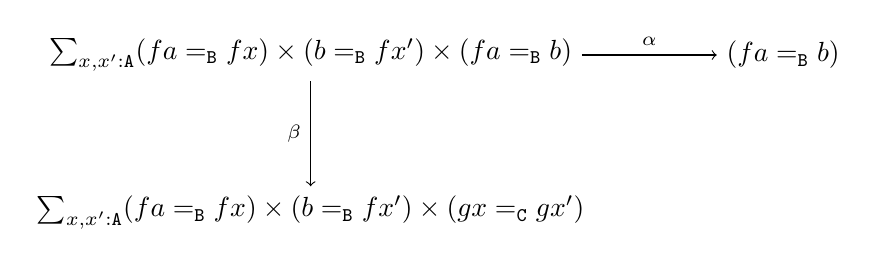
\begin{tikzpicture}
	\node (1) at (0,2) 
		{ $ \sum_{ x , x' : \A } 
			( fa =_{\B} fx ) 
			\times ( b =_{\B} fx' ) 
			\times ( fa =_{\B} b ) $ };
	\node (2) at (6,2) 
		{ $ ( fa =_{\B} b ) $ };
	\node (3) at (0,0) 
		{ $ \sum_{ x , x' : \A } 
			( fa =_{\B} fx ) 
			\times  (b =_{\B} fx' ) 
			\times ( gx =_{\C} gx') $ };
	\draw [ -> ] (1) to 
		node [above] {\scriptsize $ \alpha $} 
		(2);
	\draw [ -> ] (1) to 
		node [left] {\scriptsize $ \beta $}
		(3);
\end{tikzpicture}
\]
Clearly, \( \code ( \inr ga, \inl b ) \) it empty unless \( b =_{\B}
fa' \). The same can be said for \( \code ( \inl fa , \inl b ) \)
because the constructors of the pushout require either a populated \(
fa =_{\B} b \) or a populated \( b =_{\B} fx' \) for any \( x' : \A
\). So, we might as well assume that \( b =_{\B} fa \).  Why not \( b
=_{\B} fa' \) for some other \( a' : \A \)? I should think about this
later.

Now, we have that
\[
  \code (\inr ga, \inl fa) \coloneqq \Sigma_{x:\A} ( ga =_{\C} gx)
  \times ( fa =_{\B} fx )
\]
and
\[
  \code ( \inl fa, \inl fa)
\]
is the pushout of
\[
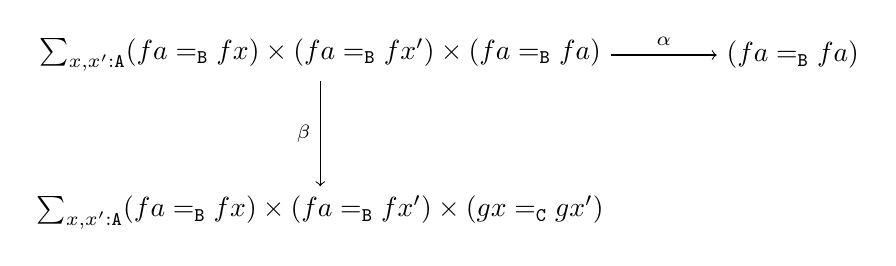
\begin{tikzpicture}
	\node (1) at (0,2) 
		{ $ \sum_{ x , x' : \A } 
			( fa =_{\B} fx ) 
			\times ( fa =_{\B} fx' ) 
			\times ( fa =_{\B} fa ) $ };
	\node (2) at (6,2) 
		{ $ ( fa =_{\B} fa ) $ };
	\node (3) at (0,0) 
		{ $ \sum_{ x , x' : \A } 
			( fa =_{\B} fx ) 
			\times  (fa =_{\B} fx' ) 
			\times ( gx =_{\C} gx') $ };
	\draw [ -> ] (1) to 
		node [above] {\scriptsize $ \alpha $} 
		(2);
	\draw [ -> ] (1) to 
		node [left] {\scriptsize $ \beta $}
		(3);
\end{tikzpicture}
\]
which should just be \( \{ \refl_{fa} \} \) since \( \B \) is a set.
It follows that \( \decode ( \code ( \inl fa , \inl fa ) ) \) maps \(
\refl_{fa} \) to \( (\refl_{fa}) \) as required.  We must now show
that \( \decode ( \code ( \inr ga , \inl fa ) ) \) is also \(
\refl_{fa} \).  But this follows from
\[
  \code ( \inr ga , \inl fa ) = (ga =_{\C} ga) \times ( fa _{\B} fa )
  = \{(\refl_{ga}, \refl_{fa})
\]
which is mapped via \( \decode \) to \( ( \ap_{\inl} \refl_{fa} ) (
\glue a ) ( \ap_{\inr} \refl_{ga} \), which is equal to \( \glue a \).
But since \( \glue a \) is contractible, it is homotopic to \( \refl_{fa} \).   

\pagebreak

% ~~~~~~~~~~~~~~~~~~~~~~~~~~~~~~~~~
% ~~~~~~~~~~~~~~~~~~~~~~~~~~~~~~~~~
% ~~~~~~~~~~~~~~~~~~~~~~~~~~~~~~~~~
% ~~~~~~~~~~~~~~~~~~~~~~~~~~~~~~~~~
% ~~~~~~~~~~~~~~~~~~~~~~~~~~~~~~~~~
% ~~~~~~~~~~~~~~~~~~~~~~~~~~~~~~~~~

\section{another shot}

This section contains the latest strategy for proving that \( \BAC \)
is a pushout.

Thus far, we've defined all of the \( \code \) spaces, and the map \(
\encode \).  It remains to define \( \decode \). To do this, we are
fixing basepoints \( \inl (b) \) and \( \inr (c) \) in the pushout
and will define
\[
  \decode ( \inl b , - ) \from
  \prod\limits_{x \tin \BAC} \code ( \inl b , x ) \to
  \inl b =_{\BAC} x
\]
and also 
\[
  \decode ( \inr c , - ) \from
  \prod\limits_{x \tin \BAC} \code ( \inr c , x ) \to
  \inr c =_{\BAC} x.
\]
Why does this work?  We've already shown that \( \code ( \inl b , x ) \)
and \( \code ( \inr c , x ) \) are propositions for any \( x \).  It
will follow that if \( \decode (\inl b , - ) \) and
\( \decode ( \inr c , - ) \) are equivalences, then we'll have that
both \( (\inl b =_{\BAC} x ) \) and \( ( \inr c =_{\BAC} x ) \) are
also propositions. But once we have that the latter are propositions,
we know that all identity spaces are propositions because any type
\( y =_{\BAC} x \) is merely equal to \( \inl b =_{\BAC} x \) or
\( \inr c =_{\BAC} x \).

\subsection{Define $ \decode ( \inl b , - ) $} %------------

To define the map

\begin{equation} \label{eq:decode-b-blank}
  \decode ( \inl b , - )
  \from
  \prod\limits_{x \tin \BAC} \code ( \inl b , x )
  \to
  \inl b =_{\BAC} x
\end{equation}

we use induction on \( \BAC \) which, in practice, means that we will
have the following two function types:
%
\begin{itemize}
\item
  \( \decode ( \inl b , - ) ( \inl b' )
  \from
  \code (\inl b , \inl b')
  \to
  ( \inl b =_{\BAC} \inl b' ) \)
\item
  \( \decode ( \inl b , - ) ( \inl c )
  \from
  \code ( \inl b , \inr c )
  \to
  ( \inl b =_{\BAC} \inr c \) 
\end{itemize}
%
and a witness

\begin{align*}
  \ap_{\decode ( \inl b , - )} (\glue a) &
  \tin
  ( \code ( \inl b , \inl fa ) \to ( \inl b =_{\BAC} \inl fa ) \\
  & =
  ( \code ( \inl b , \inl ga ) \to ( \inl b =_{\BAC} \inl ga )
\end{align*}

% question: aaosidjfpf  

\subsubsection{Define \( \decode ( \inl b , - ) ( \inl b' ) \)} %--------------------

When \( x \) is \( \inl b' \tin \BAC \), then \ref{eq:decode-b-blank} becomes
\[
  \decode ( \inl b , - )
  \from
  \code ( \inl b , \inl b' )
  \to
  \inl b =_{\BAC} \inl b'
\]
This is defined by induction on \( \code ( \inl b , \inl b' ) \)
which, recall, is the
pushout of the span
\[
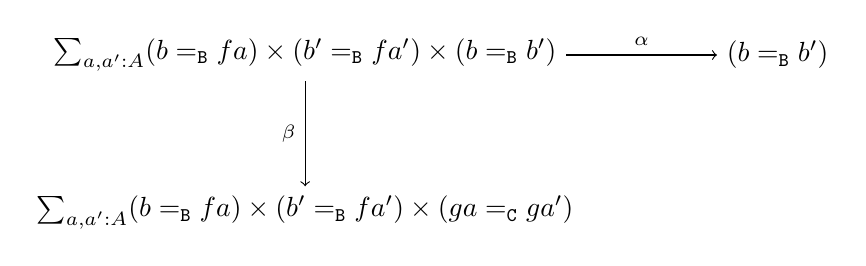
\begin{tikzpicture}
  \node (1) at (0,2) { $ \sum_{ a , a' : A }
    ( b =_\B fa ) \times ( b' =_\B fa' ) \times ( b =_\B b' ) $ };
  \node (2) at (6,2) { $ ( b =_\B b' ) $ };
  \node (3) at (0,0) { $ \sum_{ a , a' : A }
    ( b =_\B fa ) \times (b' =_\B fa' ) \times ( ga =_\C ga' ) $ };
  \draw [ -> ] (1) to node [above] {\scriptsize $ \alpha $} (2);
  \draw [ -> ] (1) to node [left] {\scriptsize $ \beta $} (3);
\end{tikzpicture}
\]
Since there are two pushouts running around, denote the inclusion maps
associated to \( \BAC \) by \( \inl \) \& \( \inr \) and denote the
inclusion maps assiciated to \( \code ( \inl b , \inl b' ) \) by \(
\inl' \) \& \( \inr' \). 

We need to define values
%
\begin{itemize}
\item
  \( \decode ( \inl b, - ) (\inl' p) \tin ( b =_{\BAC} b' ) \) for \( p
  \tin b =_{\B} b' \)
\item
  \( \decode (\inl b, - ) ( \inr' (q,r,s) ) \tin ( b ={\BAC} b' ) \)
  for
  \( (q,r,s) \tin ( b =_B fa ) \times (b' =_\B fa' ) \times ( ga =_\C
  ga' ) \)
\item
  \begin{align*}
    \ap_{\decode ( \inl b , - )} ( \glue (t,u,v) ) & \tin
    ( \decode ( \inl b, - ) ( \inl' ( \alpha (t,u,v) ) ) =_{\inl b
    =_{\BAC} \inl b'} \\
    & \decode ( \inl b, -- ) ( \inr' ( \beta (t,u,v) ) )
  \end{align*}
  for \( (t,u,v) \tin ( b =_\B fa ) \times
  ( b' =_\B fa' ) \times ( b =_\B b' ) \). 
\end{itemize}
%
These are respecively
%
\begin{itemize}
\item
  let \( \decode ( \inl b , -- ) ( \inl' p ) \) be
  \( \ap_{\inl} (p) \)
\item
  let \( \decode ( \inl b , -- ) (q,r,s) \) be the path
  \( ap_{\inl} q ; \glue a ; \ap_{\inr} s ; \glue^{-1} a' ; r^{-1} \) in
  \( \inl b =_{\BAC} \inl b' \)
\item
  we show that \( \ap_{\decode ( \inl b , -- )} (t,u,v) \) is trivial.
\end{itemize}

\begin{lemma}
  When inhabited, the type
  \[
    \type{T} \coloneqq \sum_{a,a' \tin \A} ( b =_{\B} fa ) \times ( b' =_{\B} fa' )
    \times ( b =_{\B} b' )
  \]
  is equivalent to \( \type{1} \). 
\end{lemma}

\begin{proof}
  Let \( (t,u,v) \tin \type{T} \).  Then \( t^{-1} ; v ; u \tin
  fa =_{\B} fa' \). By the injectivity of \( f \), there exists \( x
  \tin a =_{\A} a' \). We can reduce \( \type{T} \) to
  \[
    \sum_{a'',a''' \tin \A} ( fa =_{\B} fa'' ) \times ( fa' =_{\B} fa''' ) \times ( fa =_{\B} fa' ).
  \]
  The injectivity of \( f \) allows further reduction to
  \[
    ( a =_{\A} a'' ) \times ( a' =_{\A} a''' ) \times ( a =_{\A} a' ).
  \]
  This is a proposition since \( \A \) is a set, but since we are
  starting with \( \type{T} \) inhabited, we further reduce the above
  to \( \type{1} \).
\end{proof}

\begin{lemma}
  When \( \type{T} \) from above is inhabited, then \( ( b =_{\B} b' ) \sim \type{1} \). 
\end{lemma}

\begin{proof}
  Combine the two facts: \( \B \) is a set and \( \type{T} \) being
  inhabitied implies that \( b =_{\B} b' \) is inhabitied.
\end{proof}

\begin{lemma}
  When the type \( \type{T} \) from above is inhabited, the type
  \[
    \type{S} \coloneqq \sum_{a,a' \tin \A} ( b =_{\B} fa ) \times ( b' =_{\B} fa' )
    \times ( ga =_{\C} ga' )
  \]
  is equivalent to \( \type{1} \). 
\end{lemma}

\begin{proof}
  That \( \type{T} \) being inhabited implies that \( \type{S} \) is.
  But \( \type{S} \) is equivalent to
  \[
    ( fa =_{\B} fa ) \times ( fa' =_{\B} fa' ) \times ( ga =_{\C} ga' ).
  \]
  Because \( \B \) is a set, the first two factors above are
  equivalent to \( \type{1} \), whence \( \type{S} \) is equivalent to
  \( ga =_{\C} ga' \). That is inhabitied by assumption and \( \C \)
  is a set, and so it---and therefore \( \type{S} \) --- is equivalent
  to \( \type{1} \). 
\end{proof}

\begin{thm}
  When \( \type{T} \) is inhabited, \( \code ( \inl b , \inl b' ) \)
  is equivalent to \( \type{1} \).
\end{thm}

\begin{proof}
  The preceeding three lemmas imply the span over which we define \(
  \code ( \inl b , \inl b' ) \) is equivalent to the span
  \[
    \type{1} \gets \type{1} \to \type{1}
  \]
  whose pushout is \( \type{1} \).
\end{proof}

We conclude that \( \code ( \inl b , \inl b' ) \) is a 0-type and so
the relevant part of \( \decode \) is automatically continuous/functorial.

\subsubsection{Define \( \decode ( \inl b , - ) ( \inl c ) \)} %---------------------

When \( x \) is \( \inr c \tin \BAC \), then \eqref{eq:decode-b-blank} becomes
\[
  \decode ( \inl b , - )
  \from
  \code ( \inl b , \inr c )
  \to
  ( \inl b =_{\BAC} \inr c )
\]
We have that
\[
  \code ( \inl b , \inr c )
  =
  \sum\limits_{a \tin \A} (b =_{\B} fa) \times (c =_{\C} ga)
\]
Define
\[
  \decode ( \inl b , - ) ( p , q )
  \coloneqq
  \inl p ; \glue a ; \inr q
\]

\subsubsection{ Define \( \ap_{\decode ( \inl b , - )} (\glue a) \) } %------------------

Right now, we define

\begin{align*}
  \ap_{\decode ( \inl b , - )} (\glue a) &
  \tin
  ( \code ( \inl b , \inl fa ) \to ( \inl b =_{\BAC} \inl fa ) \\
  & =
  ( \code ( \inl b , \inl ga ) \to ( \inl b =_{\BAC} \inl ga )
\end{align*}

To define this is to construct a commuting square
\[
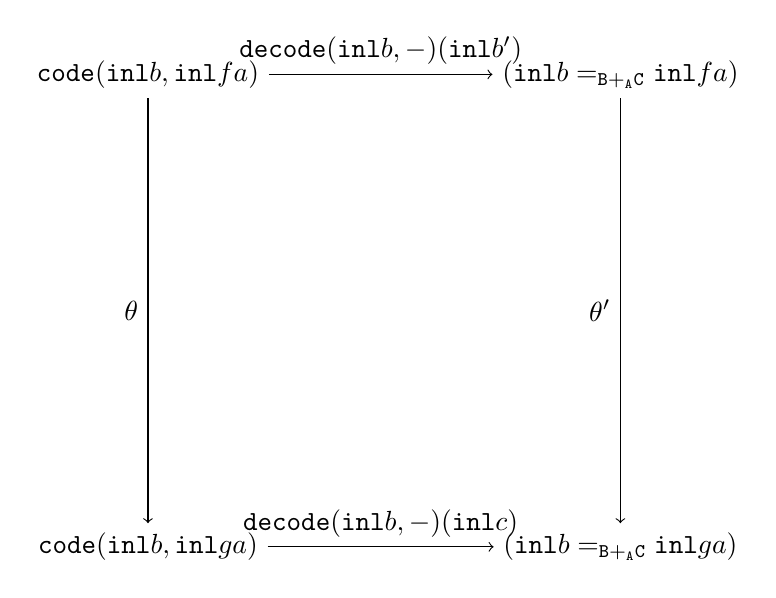
\begin{tikzpicture}
  \node (code-bb) at (-3,3) {\( \code ( \inl b , \inl fa ) \)};
  \node (code-bc) at (-3,-3) {\( \code ( \inl b , \inl ga ) \)};
  \node (id-bb) at (3,3) {\( ( \inl b =_{\BAC} \inl fa ) \)};
  \node (id-bc) at (3,-3) {\( ( \inl b =_{\BAC} \inl ga ) \)};
  \draw [->] (code-bb) to node [left] {\( \theta \)} (code-bc);
  \draw [->] (code-bb) to node [above] {\( \decode (\inl b,-)(\inl b') \)} (id-bb);
  \draw [->] (id-bb) to node [left] {\( \theta' \)} (id-bc);
  \draw [->] (code-bc) to node [above] {\( \decode (\inl b,-)(\inl c) \)} (id-bc);
\end{tikzpicture}
\]
We have already defined the two \( \decode \) maps. The map \( \theta'
\) is post-composition by \( \glue a \). The map \( \theta \) requires
induction to define because we are mapping out of a pushout.
Therefore, we need the following three values to define \( \theta \):
\begin{itemize}
\item \( \theta (\inl' p) \) for \( p \tin b=_Bfa \)
\item \( \theta ( \inr' (q,r,s) ) \) for \( (q,r,s) \tin
  \sum\limits_{a',a'' \tin \A} (b=_\B fa') \times (fa =_B fa'') \times
  (ga' =_C ga'') \) 
\item \( \ap_{ \theta } ( \glue (t,u,v) ) \tin \theta ( \inl' (\alpha
  (t,u,v) ) ) = \theta ( \inr' ( \beta (t,u,v) ) ) \).
\end{itemize}

A quick remark on notation: since \( f \) is monic and \( \B \) is a
set, we can pull back any paths of form \( r \tin fa =_\B fa'\) to a
path \( \hat{r} \tin a =\A a' \).

Define \( \theta (\inl' p) \) for \( p \tin b=_Bfa \) to
be \( ( p , \refl_{ga} ) \). Define \( \theta ( q,r,s ) \) to be \( (
q , \ap_g ( \hat{r} ) ; s^{-1} ) \).

Now we know that \( \ap_{ \theta } ( \glue ( t,u,v ) ) \) is a path from
\(\theta ( \inl' ( v ) ) = ( v , \refl_{ga} ) \) to \( \theta ( \inr'
( \beta ( t,u,v ) ) ) = \theta ( \inr' ( t,u,\ap_{g}(\hat{v}) ) ) = (
t,\ap_g ( \hat{u} ); \ap_g ( \hat{v} )^{-1} ) = ( t, \ap_g ( \hat{u} ;
\hat{v}^{-1}) ) \). With this in mind, we will define \( \ap_{\theta}
( \glue ( t,u,v ) ) \) to be post-composition by
\[
  ( \ap_f ( \hat{u};\hat{v}^{-1} ) , \ap_g ( \hat{u};\hat{v}^{-1} ) ).
\]

Now we need to check that the diagram commutes.  Since \( \code ( \inl
b , \inl fa ) \) is a set, it suffices to check that
\[
  \theta' ( \decode (\inl b,-) ( \inl fa ) ( x ) )
  =_{ \inl b =_{\BAC} \inr ga }
  \decode ( \inl b,-)(\inr ga) ( \theta ( x ) )
\]
where \( x \tin \code ( \inl b, \inl fa ) \) is
\begin{itemize}
\item
  \( \inl' p \) for \( p \tin b=_\B fa \), and
\item
  \( \inr' ( q,r,s ) \) for
  \( ( q,r,s ) \tin \sum\limits_{a',a'' \tin \A} (b=_\B fa') \times (
  fa =_\B fa'' )\times ( ga'=_\C ga'' ) \)
\end{itemize}
and we also need to check that
\[
  \ap_{\theta' ; \decode (\inl b,-) ( \inl fa ) )} ( \glue ( t,u,v ) ) 
  =_{ \inl b =_{\BAC} \inr ga }
  \ap_{ \decode ( \inl b,-)(\inr ga) ; \theta } ( \glue ( t,u,v ) ) 
\]

Set \( x \coloneqq \inl' p \).  Then
\begin{align*}
  \theta' ( \decode (\inl b,-) ( \inl fa ) ( \inl' p ) )
  & = \theta' ( ( \ap_{\inl'} p ) ) \\
  & = \ap_{\inl'} p ; \glue a
\end{align*}
Also,
\begin{align*}
  \decode ( \inl b , - ) ( \inr ga ) ( \theta ( \inl' p ) )
  & = \decode ( \inl b , - ) ( \inr ga ) ( ( p,\refl_{ga} ) ) \\
  & = \ap_{\inl'} p ; \glue a ; \ap_{\inr'} \refl_{ga} \\
  & = \ap_{\inl'} p ; \glue a ; \refl_{\inr' ga} \\
  & = \ap_{\inl'} p ; \glue a
\end{align*}
Therefore, the square commutes on \( \inl' p \)

Set \( x \coloneqq \inr' ( q,r,s ) \). Then
\begin{align*}
  \theta' ( \decode (\inl b,-) ( \inl fa ) ( \inr' ( q,r,s ) ) )
  & = \theta' ( \ap_{\inl} q ; \glue a' ; \ap_{\inr} s ; \glue a'' ;
    \ap_{\inl} r^{-1} ) \\
  & =  \ap_{\inl} q ; \glue a' ; \ap_{\inr} s ; \glue^{-1} a'' ;
    \ap_{\inl} r^{-1} ; \glue a \\
   & =  \ap_{\inl} q ; \glue a' ; \ap_{\inr} s ; \glue^{-1} a'' ;
    \ap_{\inl} \ap_f \hat{r}^{-1} ; \glue a \\
\end{align*}
Also,
\begin{align*}
  \decode ( \inl b , - ) ( \inr ga ) ( \theta ( \inr' ( q,r,s ) ) )
  & = \decode ( \inl b , - )( \inr ga )( q , \ap_g ( \hat{r} ; s^{-1}
    ) ) \\
  & = \ap_{\inl} q ; \glue a' ; ( \ap_{\inr} ( \ap_g \hat{r} ; s^{-1} )^{-1} ) \\
  & = \ap_{\inl} q ; \glue a' ; \ap_{\inr} ( \ap_g ( \hat{r} ) ; ( \ap_g
    (s^{-1}) )^{-1} ) \\
  & = \ap_{\inl} q ; \glue a' ; \ap_{\inr} (s^{-1})^{-1} ;  \ap_g ( \hat{r} )^{-1} \\
  & = \ap_{\inl} q ; \glue a' ; \ap_{\inr} (s^{-1})^{-1} ;  \ap_g ( \hat{r} )^{-1} \\
  & = \ap_{\inl} q ; \glue a' ; \ap_{\inr} s ;  \ap_g ( \hat{r} )^{-1} \\
\end{align*}
We just need to check that
\[
  \ap_g ( \hat{r} )\inv = \glue\inv a'' ; \ap_{ \inl } \ap_f
  \hat{r}\inv ; \glue a
\]
But this follows from the continuity of \( \glue \), that is, it
preserves paths. Therefore, the square commutes on \( \inr' ( q,r,s )
\).

It remains to check that
\[
  \ap_{\theta' ; \decode (\inl b,-) ( \inl fa ) )} ( \glue ( t,u,v ) ) 
  =_{ \inl b =_{\BAC} \inr ga }
  \ap_{ \decode ( \inl b,-)(\inr ga) ; \theta } ( \glue ( t,u,v ) ) 
\]
for \( ( t,u,v ) \tin \sum\limits_{a',a''\tin \A} ( b =_\B fa' )
\times ( fa =_\B fa'' ) \times ( b =_{\B} fa ) \). Here, we make some
reductions.
\begin{itemize}
\item Because \( f \) is monic, we get that \( fa =_\B fa'' \) reduces
  to \( fa =_\B fa \). Since \( \B \) is a set, we can take \( u =
  \refl_{fa} \).
\item The type \( b =_\B fa' \) reduces to \( fa =_\B fa \) because \(
  \B \) is monic, so \( t = \refl_{fa} \).
\item The type \( b =_\B fa \) reduces to \( fa =_\B fa \) because \(
  \B \) is monic, so \( v = \refl_{fa} \).
\end{itemize}
Hence without loss of generality, we can take \( ( t,u,v ) = ( \refl_{fa},\refl_{fa},\refl_{fa} ) \).
Therefore, it suffices to check that 
\[
  \ap_{\theta' ; \decode (\inl b,-) ( \inl fa ) )} ( \glue ( \refl_{fa},\refl_{fa},\refl_{fa} ) ) 
  =_{ \inl b =_{\BAC} \inr ga }
  \ap_{ \decode ( \inl b,-)(\inr ga) ; \theta } ( \glue ( \refl_{fa},\refl_{fa},\refl_{fa} ) ). 
\]
But because the square commutes on points as shown above, the two
paths on the left and right of the above equation are certainly
parallel.  Then functorality gives us that \( \refl_{fa} \) is
preserved. Hence the square commutes.

%~~~~~~~~~~~~~~~
%~~~~~~~~~~~~~~~
%~~~~~~~~~~~~~~~
%~~~~~~~~~~~~~~~

\subsection{Define decode(c,-)}

To define the map

\begin{equation} \label{eq:decode-b-blank}
  \decode ( \inr c , - )
  \from
  \prod\limits_{x \tin \BAC} \code ( \inr c , x )
  \to
  \inr c =_{\BAC} x
\end{equation}

we use induction on \( \BAC \) which, in practice, means that we will
have the following two function types:
%
\begin{itemize}
\item
  \( \decode ( \inr c , - ) ( \inl b )
  \from
  \code (\inr c , \inl b)
  \to
  ( \inr c =_{\BAC} \inl b ) \)
\item
  \( \decode ( \inr c , - ) ( \inr c' )
  \from
  \code ( \inr c , \inr c' )
  \to
  ( \inr c =_{\BAC} \inr c' \) 
\end{itemize}
%
and a witness

\begin{align*}
  \ap_{\decode ( \inr c , - )} (\glue a) &
  \tin
  ( \code ( \inr c , \inl fa ) \to ( \inr c =_{\BAC} \inl fa ) \\
  & =
  ( \code ( \inr c , \inl ga ) \to ( \inr c =_{\BAC} \inl ga )
\end{align*}

\subsubsection{Define \( \decode ( \inr c , - ) ( \inl b ) \)} %--------------------

Here, we define a map
\[
  \decode ( \inr c , - ) ( \inl b )
  \from
  \code ( \inr c , \inl b )
  \to
  ( \inr c =_{\BAC} \inl b ).
\]
Recall that \( \code ( \inr c , \inl b ) \coloneqq \sum\limits_{a \tin
\A} ( c =_{\C} ga ) \times ( b =_{\B} fa ) \). Thus for any \( ( p,q )
\) in \( \code ( \inr c , \inl b ) \), we define a path \( \decode (
\inr c , - ) ( \inl b ) ( p,q ) \) in \( \BAC \) from \( \inr c \) to
\( \inl b \).  Take this path to be \( \inr p ; \glue^{-1}  a ; \inl q^{-1} \).

\subsubsection{Define \( \decode ( \inr c , - ) ( \inr c' ) \)} %--------------------

Here, we define a map
\[
  \decode ( \inr c , - ) ( \inr c' )
  \from
  \code ( \inr c , \inr c' )
  \to
  ( \inr c =_{\BAC} \inr c' ).
\]
Recall that
\[
  \code ( \inr c , \inr c' ) \coloneqq
  \sum\limits_{a \tin \A}
  ( c =_{\C} ga ) \times ( c' =_{\C} ga' ) \times ( fa =_{\B} fa' ) 
\]
Thus for any \( ( p,q,r ) \) in \( \code ( \inr c , \inr c' ) \), we define a path \( \decode (
\inr c , - ) ( \inr c' ) ( p,q,r ) \) in \( \BAC \) from \( \inr c \) to
\( \inr c' \).  Take this path to be \( \inr p ; \glue\inv a ; \inl r
\glue a' ; \inr q\inv \).

\subsubsection{Define \( \ap_{\decode ( \inr c , - )} (\glue a) \)} %--------------------

Here, we define a path
\begin{align*}
  \ap_{\decode ( \inr c , - )} (\glue a) &
  \tin
  ( \code ( \inr c , \inl fa ) \to ( \inr c =_{\BAC} \inl fa ) \\
  & =
  ( \code ( \inr c , \inl ga ) \to ( \inr c =_{\BAC} \inl ga ).
\end{align*}
Placing the definitions in for the two \( \code \) expressions, this
path is constructed as a commuting square
\[
  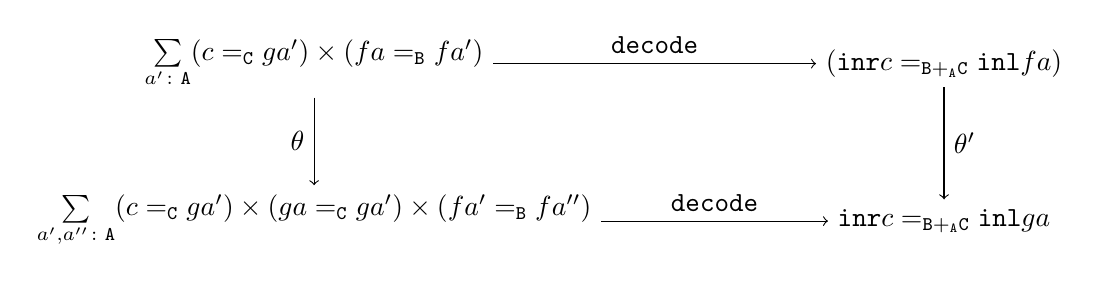
\begin{tikzpicture}
    \node (1) at (-4,1) {\( \sum\limits_{a' \tin \A} ( c =_{\C} ga' )
      \times ( fa =_{\B} fa' ) \)};
    \node (2) at (-4,-1) {\( \sum\limits_{a',a'' \tin \A} ( c =_{\C}
      ga' ) \times ( ga =_{\C} ga' ) \times ( fa' =_{\B} fa'' ) \)};
    \node (3) at (4,1) {\( ( \inr c =_{\BAC} \inl fa ) \)};
    \node (4) at (4,-1) {\( \inr c =_{\BAC} \inl ga \)};
    \draw [->] (1) to node [left] {\( \theta \)} (2);
    \draw [->] (1) to node [above] {\( \decode \)} (3);
    \draw [->] (2) to node [above] {\( \decode \)} (4);
    \draw [->] (3) to node [right] {\( \theta' \)} (4); 
  \end{tikzpicture}
\]
The easier to define is \( \theta' \) which is simply concatenation
with \( \glue a \).  To define \( \theta \), we send \( ( p,q )
\mapsto ( p, \refl_{ga} , q ) \).  Now we need to see if this square
commutes. We have that
\begin{align*}
  \theta' ( \decode ( \inr c , - ) ( \inl fa ) ( p,q ) )
  & = \theta' ( \inr p ; \glue^{-1} a' ; \inl q^{-1}  ) \\
  & = \inr p ; \glue^{-1} a' ; \inl q^{-1} ; \glue a. \\
\end{align*}
We also have that
\begin{align*}
  \decode ( \inr c , - ) ( \inl ga ) ( \theta ( p,q ) )
  & = \decode ( \inr c , - ) ( \inl ga ) ( p,\refl_{ga},q ) \\
  & =  \inr p ; \glue\inv a' ; \inl q\inv ; \glue a ; \inr \refl_{ga} \\
  & =  \inr p ; \glue\inv a' ; \inl q\inv ; \glue a  \\
\end{align*}
Hence the square commutes.

% ~~~~~~~~~~~~~~~~~~~~~~~~~~~~~~
% ~~~~~~~~~~~~~~~~~~~~~~~~~~~~~~
% ~~~~~~~~~~~~~~~~~~~~~~~~~~~~~~
% ~~~~~~~~~~~~~~~~~~~~~~~~~~~~~~

\section{Composing encode and decode}

Let's compose \( \encode \) and \( \decode \) maps to see if they are
mutual inverses.  

\edit{ Are we required to define this using induction on the pushout
  or no? We've already defined encode and decode, so maybe it's
  unnecessary. For now, I'll include both.}

\subsection{encode;decode with induction}

First, we look at the composite
\[
  \encode ; \decode
  \from
  \prod\limits_{x,y \tin \BAC} x =_{\BAC} y
  x =_{\BAC} y
\]

% THE FOLLOWING PARAGRAPH NEEDS TO BE JUSTIFIED W MIKES EMAIL
This map can be computed using single, as opposed to double, induction
on \( \BAC \). That is, we can instead compute values
\begin{itemize}
\item
  \( \encode ; \decode ( \inl b , - ) \from \prod\limits_{x \tin
  \BAC} ( \inl b =_{\BAC} x ) \to ( \inl b =_{\BAC} x ) \)
\item
  \( \encode ; \decode ( \inr c , - ) \from \prod\limits_{x \tin
  \BAC} \inr c =_{\BAC} x \to ( \inr c =_{\BAC} x ) \)
\item
  \( \ap_{\encode ; \decode} (\glue a ) \tin \encode ; \decode ( \inl
  fa , -  )
  =_{\BAC} \encode ; \decode (\inr ga , - ) \)
\end{itemize}

The first two of these will be computed using induction on \( \BAC
\). To check \( \encode ; \decode ( \inl b , - ) \), we need the
following:
\begin{itemize}
\item
  \( \encode ; \decode ( \inl b , - ) ( \inl b' ) \from ( \inl b
  =_{\BAC} \inl b' ) \to ( \inl b =_{\BAC} \inl b' )  \). By path
  induction, suffice to check \( \refl_{\inl b} \):
  \[
    \refl_{\inl b} \mapsto \ap_{\inl'} \refl_{\inl b}
    = \refl_{\inl' b} \mapsto \ap_{\inl} \refl_{\inl' b} =
    \refl_{\inl b}.
  \]
  So this one checks out.
\item
  % CHECK THAT GLUE IS THE ONLY THING IN fa=ga
  \( \encode ; \decode ( \inl b , - ) ( \inl b' ) \from ( \inl b
  =_{\BAC} \inr c ) \to ( \inl b =_{\BAC} \inr c )  \). This is only
  non-trivial when \( b =_\B fa \) and \( c =_\C ga \). Hence
  \[
    \glue a \mapsto ( \refl_{fa} , \refl_{ga} ) \mapsto \ap_{\inr}
    \refl_{ga} ; \glue a ; \ap_{\inl} \refl_{fa} = \glue a.
  \]
  This one checks out too.
\item
  % AM I LEVEL SLIPPING HERE? 
  \( \ap_{\encode ; \decode ( \inl b, -)} (\glue a) \encode ; \decode
  (\inl b , -)(\inl fa) = \encode ; \decode (\inl b , -)(\inr ga)
  \). Note that the left hand side of this path space lives in
  \[
    \inl b =_{\BAC} \inl fa
  \]
  and the righthand side lives in
  \[
    \inl b =_{\BAC} \inr ga
  \]
  There is an equivalence between these path spaces obtained by
  concatenating \( \glue a \) and its inverse. Applying univalence to
  this equivalence gives us \( \ap_{\encode ; \decode (\inl b , )}
  \glue a \).
\end{itemize}

That completes the definition of \( \encode ; \decode (\inl b, -)
\). Now, move on to \( \encode ; \decode ( \inr c, - ) \), which as we
are inducting over \( \BAC \), requires obtaining three values:
\begin{itemize}
\item
  \( \encode ; \decode ( \inr c , - ) ( \inl b ) \from ( \inr c
  =_{\BAC} \inl b ) \to ( \inr c =_{\BAC} \inl b )  \). This is
  symmetric to the above case, so checks out. 
\item
  \( \encode ; \decode ( \inr c , - ) ( \inr c' ) \from ( \inr c
  =_{\BAC} \inr c' ) \to ( \inr c =_{\BAC} \inr c' )  \). By path
  induction, that
  \[
    \refl_{\inr c} \mapsto \refl_c \mapsto \ap_{\inr} \refl_c =
    \refl_{\inr c}
  \]
  suffices.  
\item
  \( \ap_{\encode ; \decode ( \inr c, -)} (\glue a) \tin \encode ; \decode
  (\inl b , -)(\inl fa) = \encode ; \decode (\inr c , -)(\inr ga)
  \).  Note that the left hand side of this path space is
  \[
    \inr c =_{\BAC} \inl fa
  \]
  and the righthand side is
  \[
    \inr c =_{\BAC} \inr ga
  \]
  There is an equivalence between these path spaces obtained by
  concatenating \( \glue a \) and its inverse. Applying univalence to
  this equivalence gives us \( \ap_{\encode ; \decode (\inr c , )}
  \glue a \).
\end{itemize}

The final thing to construct is a path
\( \ap_{\encode ; \decode} (\glue a ) \tin \encode ; \decode ( \inl fa
, - ) =_{\BAC} \encode ; \decode (\inr ga , -) \). Univalence allows
us to instead find and equivalence
\[
  \prod\limits_{x \tin \BAC} ( \inl fa =_{\BAC} x )
  \simeq
  \prod\limits_{x \tin \BAC} ( \inr ga =_{\BAC} x )
\]
This equivalence is obtained by concatenation by \( \glue a \) and its
inverse.

And so, we have prove that \( \decode \) is a section for \( \encode
\). The opposite direction remains.

\subsection{encode;decode without induction}

First, we look at the composite
\[
  \encode ; \decode
  \from
  \prod\limits_{x,y \tin \BAC} x =_{\BAC} y
  x =_{\BAC} y
\]

To show that this map is the identity up to homotopy, we compute two values:
\begin{itemize}
\item
  \( \encode ; \decode ( \inl b , - ) \from \prod\limits_{x \tin
  \BAC} ( \inl b =_{\BAC} x ) \to ( \inl b =_{\BAC} x ) \)
\item
  \( \encode ; \decode ( \inr c , - ) \from \prod\limits_{x \tin
  \BAC} \inr c =_{\BAC} x \to ( \inr c =_{\BAC} x ) \)
\end{itemize}

but computing these values actually requires the computation of the
following four maps:
\begin{itemize}
\item
  \( \encode ; \decode ( \inl b , - )(\inl b') \from \code ( \inl b ,
  \inl b' ) \to ( \inl b =_{\BAC}
  \inl b' ). \) By path
  induction, it suffices to check \( \refl_{\inl b} \):
  \[
    \refl_{\inl b} \mapsto \ap_{\inl'} \refl_{\inl b}
    = \refl_{\inl' b} \mapsto \ap_{\inl} \refl_{\inl' b} =
    \refl_{\inl b}.
  \]
  So this one checks out.
\item
  \( \encode ; \decode ( \inl b , - )(\inr c) \from \code ( \inl b ,
  \inr c ) \to ( \inl b =_{\BAC} \inl c ) \). \edit{glue(a) *is* the
    only thing to check here, right?} This is only non-trivial when
  \( b =_\B fa \) and \( c =_\C ga \). Hence
  \[
    \glue a \mapsto ( \refl_{fa} , \refl_{ga} ) \mapsto \ap_{\inr}
    \refl_{ga} ; \glue a ; \ap_{\inl} \refl_{fa} = \glue a.
  \]
  This one checks out too.
\item
  \( \encode ; \decode ( \inr c , - )(\inl b) \from \code ( \inr c ,
  \inl b ) \to ( \inr c =_{\BAC} \inl b ) \). This is
  symmetric to the above case, so checks out. 
\item
  \( \encode ; \decode ( \inr c , - )(\inr c') \from \code ( \inr c,
  \inr c' ) \to ( \inr c =_{\BAC} \inr c' ) \). By path
  induction, 
  \[
    \refl_{\inr c} \mapsto \refl_c \mapsto \ap_{\inr} \refl_c =
    \refl_{\inr c}
  \]  
\end{itemize}

And so, we have prove that \( \decode \) is a section for \( \encode
\). The opposite direction remains.

\subsection{decode;encode}

Now, we look at the composite
\[
  \decode ; \encode
  \from
  \prod\limits_{x,y \tin \BAC} \code ( x,y )
  \to
  \code ( x,y )
\]
We can compute this composite by computing values

\begin{itemize}
\item
  \( \decode ; \encode (\inl b , -) ( \inl b' ) \from \code ( \inl b ,
  \inl b' ) \to \code ( \inl b , \inl b' ) \)
\item
  \( \decode ; \encode (\inl b , -) ( \inr c ) \from \code ( \inl b ,
  \inr c ) \to \code ( \inl b , \inr c ) \)
\item
  \( \decode ; \encode (\inr c , -) ( \inl b ) \from \code ( \inr c ,
  \inl b ) \to \code ( \inr c , \inl b ) \)
\item
  \( \decode ; \encode (\inr c , -) ( \inr c' ) \from \code ( \inr c ,
  \inr c' ) \to \code ( \inr c , \inr c' ) \)
\end{itemize}

But these maps are all identity since \( \code (x,y) \) is a
proposition for \( x,y \tin \BAC \).   

% ~~~~~~~~~~~~~~~~~~~~~~~~
% ~~~~~~~~~~~~~~~~~~~~~~~~
% ~~~~~~~~~~~~~~~~~~~~~~~~
% ~~~~~~~~~~~~~~~~~~~~~~~~

\section{The 'pushout is a set' theorem presented}

This section is devoted to proving the following theorem.

\begin{thm} \label{thm:pushout-is-set}
  Given mere sets \( \A \), \( \B \), and \( \C \) configured in a
  span
  \[
    \C \xgets{g} \A \xto{f} \B
  \]
  where \( f \) is monic, then the pushout \( \BAC \) is a mere set.
\end{thm}

For the remainder of the section, we denote the canonical pushout maps
as
%
\(
  \inl \from \B \to \BAC
\)
%  
and
%
\(
  \inr \from \C \to \BAC.
\)
%
\par

Consider the types
%
\(
  \P \bydef
  \{ (x,y) \tin ( \BAC ) \times ( \BAC ) \vert
  x =_{\BAC} y \text{ is a mere proposition} \}
\)
%
and 
%
\(
  \Q \bydef (\BAC) \times (\BAC).
\)
%
To prove the theorem, it is sufficient to show that the inclusion
%
\(
  \P \hookrightarrow \Q
\)
%
is an equivalence. 

% ~~~~~~~~~~~~~~~~~~~

\begin{lemma} \label{thm:inclusion-is-embedding}
%
  The inclusion
  %
  \(
    \P \to \Q
  \)
  %
  is an embedding.
%
\end{lemma}
\begin{proof}
%
  We need to show that, for each
  %
  \(
     ( x_0 , y_0 ) \tin \Q,
  \)
  % 
  the homotopy fibre
  %
  \[
     \type{F} \bydef
     \sum\limits_{ ( x,y ) \tin \P}
     ( x,y ) =_{\Q} ( x_0,y_0 )
  \]
  %
  is a mere proposition. Any
  \(
    p \tin \type{F},
  \)
  is a pair of paths
  \(
    p_x \tin x =_{\BAC} x_0
  \)
  and
  \(
    p_y \tin y =_{\BAC} y_0.
  \)
  The existance of such a $p$ implies that 
  \(
    ( x_0,y_0 ) \tin \P
  \)
  by $ \beta $-reducing $ (x,y) $ to $ ( x_0,y_0 ) $. Therefore,
  \(
    \refl_{ ( x_0,y_0 ) } \tin \type{F}.
  \)
  The cube of paths
    \[
      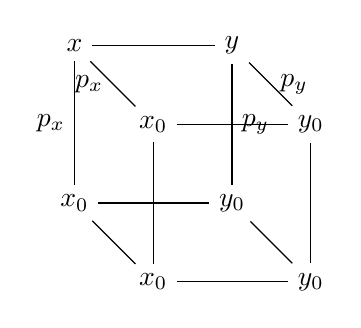
\begin{tikzpicture}
        \node (1) at (0,2) {\( x \)};
        \node (2) at (2,2) {\( y \)};
        \node (3) at (1,1) {\( x_0 \)};
        \node (4) at (3,1) {\( y_0 \)};
        \node (5) at (0,0) {\( x_0 \)};
        \node (6) at (2,0) {\( y_0 \)};
        \node (7) at (1,-1) {\( x_0 \)};
        \node (8) at (3,-1) {\( y_0 \)};
        \draw [-] (1) to (2);
        \draw [-] (3) to (4);
        \draw [-] (5) to (6);
        \draw [-] (7) to (8);
        \draw [-] (1) to node [left] {\( p_x \)} (3);
        \draw [-] (2) to node [right] {\( p_y \)} (4);
        \draw [-] (5) to (7);
        \draw [-] (6) to (8);
        \draw [-] (1) to node [left] {\( p_x \)} (5);
        \draw [-] (2) to node [right] {\( p_y \)} (6);
        \draw [-] (3) to (7);
        \draw [-] (4) to (8); 
      \end{tikzpicture}
    \]
    commutes trivially and is filled because \( \BAC \) is at most a
    1-type. Hence, we have that
    %
    \(
       p =_{ \type{F} } \refl_{ ( x_0,y_0 ) }
    \)
    %
    and \( \type{F} \) is contractible.
    \par

    \edit{Where do we use that 'being a proposition' is a
      proposition?}
%
\end{proof}

% ~~~~~~~~~~~~~~~~~~~

To prove that
%
\( 
   \P \hookrightarrow \Q
\)
%
is an equivalnece, it remains to show that \( \P \) contains a point
in every connected component of \( \Q \). Note that every connected
component of \( \BAC \) contains a point of form \( \inl b \) or
\( \inr c \). Therefore, if
%
\(
   \inl b =_{\BAC} x
\)
%
and
%
\(
   \inr c =_{\BAC} x
\)
%
are always mere propositions, then \( \P \) contains a point in every
component of \( \Q \) as desired.
\par

To actually do this, we employ the \textit{encode-decode method}. The
strategy is to introduce types
%
\(
   \prod\limits_{ x \tin \BAC} \code ( \inl b , x )
\)
%
and
%
\(
   \prod\limits_{ x \tin \BAC } \code ( \inl c , x ).
\)
%
After showing these are mere propositions---an easier task than
proving the identity types in \( \BAC \) are mere propositions---we build
an equivalence between
%
\(
   \prod\limits_{ x \tin \BAC } \code ( \inl b , x )
\)
%
and
%
\(
   \prod\limits_{ x \tin \BAC } \inl b =_{\BAC} x,
\)
% 
and likewise between
%
\(
   \prod\limits_{ x \tin \BAC } \code ( \inr c , x )
\)
%
and
%
\(
   \prod\limits_{ x \tin \BAC } \inr c =_{\BAC} x.
\)

% ~~~~~~~~~~~~~~~~~~~~~
% ~~~~~~~~~~~~~~~~~~~~~

\subsection{Defining \( \prod\limits_{x \tin \BAC} \code ( \inl b , x ) \)} 
\label{sec:define-code-bx}

To define \( \prod\limits_{ x \tin \BAC } \code ( \inl b , x ) \), we
induct on \( x \), which requires the values
%
\begin{itemize}
\item
  \(
      \code ( \inl b ,\inl b' ),
  \)
\item
  \(
      \code ( \inl b , \inr c ),
  \)
  and
\item
  \(
      \code ( \inl b , \glue a ).
  \)
\end{itemize}
%
We also show that the first two are mere propositions.  

Define
\(
    \code ( \inl b , \inl b' )
\)
as the pushout of the span
%
\[
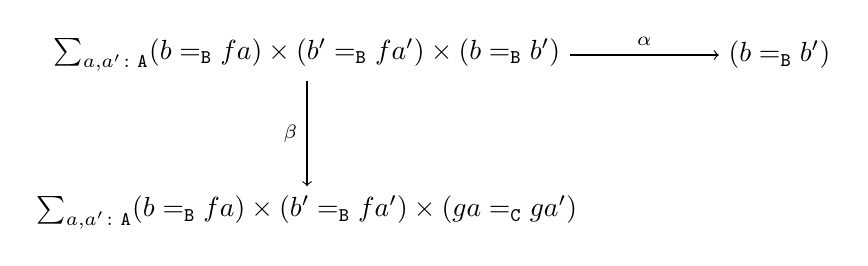
\begin{tikzpicture}
	\node (1) at (0,2) 
		{ $ \sum_{ a , a' \tin \A } 
			( b =_\B fa ) 
			\times ( b' =_\B fa' ) 
			\times ( b =_\B b' ) $ };
	\node (2) at (6,2) 
		{ $ ( b =_\B b' ) $ };
	\node (3) at (0,0) 
		{ $ \sum_{ a , a' \tin \A } 
			( b =_\B fa ) 
			\times  (b' =_\B fa') 
			\times ( ga =_\C ga' ) $ };
	\draw [ -> ] (1) to 
		node [above] {\scriptsize $ \alpha $} 
		(2);
	\draw [ -> ] (1) to 
		node [left] {\scriptsize $ \beta $}
		(3);
\end{tikzpicture}
\quad \quad 
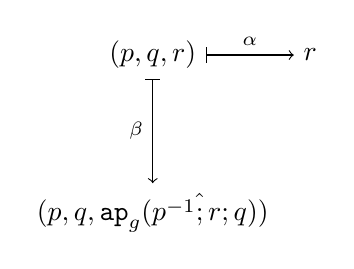
\begin{tikzpicture}
	\node (1) at (0,2) { \( ( p,q,r )  \) };
	\node (2) at (2,2) { \( r \) };
	\node (3) at (0,0) { \( ( p,q, \ap_g (\hat{p\inv ; r ; q})) \)};
        \draw [ |-> ]
          (1) to 
	  node [above] {\scriptsize $ \alpha $} 
	  (2);
        \draw [ |-> ]
          (1) to 
	  node [left] {\scriptsize $ \beta $}
	  (3);
\end{tikzpicture}
\]
%
where
\(
    \hat{p\inv ; r ; q}
\)
is the preimage of the path
%
\(
    p\inv ; r ; q \tin
    fa =_{\B} fa'
\)
% 
Its existance and uniqueness follows from
the injectivity of \( f \).
\par

To distinguish these pushout maps from those associated to \( \BAC \),
we denote them by \( \inl' \) and \( \inr' \).
\par

In the following lemma, we use the denotation
\(
    \type{X} \bydef
    \sum_{ a , a' : \A }
    ( b =_\B fa ) \times ( b' =_\B fa') \times ( ga =_\C ga' ),
\)
%
\(
    \type{Y} \bydef
    \sum_{ a , a' : \A }
    ( b =_\B fa ) \times ( b' =_\B fa' ) \times ( b =_/B b' ),
\)
%
and
%
\(
    \type{Z} \bydef b =_\B b'.
\)
\par

% ~~~~~~~~~~~~~~~~~~~

\begin{lemma} \label{thm:code-bb-isProp}
%
  The type
  \(
      \code ( \inl b , \inl b' )
  \)
  is a mere proposition.
%  
\end{lemma}
\begin{proof}
%  
  The feet of the span are mere propositions; \( \type{Z} \) trivially
  so. Showing that \( \type{X} \) is also a mere proposition requires
  some work. Pick
  \(
      ( r,s,t ) \tin
      ( b =_\B fa ) \times ( b' =_\B fa') \times ( ga =_\C ga' )
  \)
  and
  \(
      ( r',s',t' ) \tin
      ( b =_\B fa'' ) \times ( b' =_\B fa''') \times ( ga'' =_\C ga'''').
  \)
  Then
  %
  \(
      r\inv ; r' \tin fa =_\B fa''
  \)
  %
  and
  %
  \(
      s\inv ; s' \tin fa' =_\B fa''',
  \)
  %
  along with the injectivity of \( f \), ensure the existance of paths
  \(
      \hat{r} \tin a =_\A a''
  \)
  and
  \(
      \hat{s} \tin a' =_\A a'''.
  \)
  Beta-reduction provides that
  \(
      ( b =_\B fa ) \times ( b' =_\B fa') \times ( ga =_\C ga' )
  \)
  is equivalent to
  \(
     ( b =_\B fa'' ) \times ( b' =_\B fa''') \times ( ga'' =_\C ga'''' ),
  \)
  both of which are contractable because \( \B \) and \( \C \)
  are mere sets.  It follows that
  \(
      ( r,s,t ) = ( r',s',t' ).
  \)
  \par

  If
  \(
      \code ( \inl b , \inl b' )
  \)
  is not empty, then one of the span's feet must also be
  non-empty.  This leads to three cases:
  %
  \begin{itemize}
  \item
    \( \type{X} \) is empty and \( \type{Z} \) is non-empty. This
    forces \( \type{Y} \) to also be empty and so the lemma holds;
  \item
    \( \type{X} \) is non-empty and \( \type(Z) \) is empty. This
    again forces \( \type{Y} \) to be empty, so the lemma holds;
  \item
    \( \type{X} \) and \( \type{Z} \) are non-empty. It is quick to check
    that this forces \( \type{Y} \) to be non-empty. We dedicate the
    remainder of this proof to showing \( \code ( \inl b , \inl b' )
    \) is a proposition in this case.
  \end{itemize}
  %
  
  A point in the apex of the span provides a witness to
  \(
      fa =_\B fa'
  \)
  which in turn provides a witness to
  \(
      a =_\A a'.
  \)
  Beta-reduction plus univalence equates
  \[
    \type{Y} =
    \sum\limits_{a \tin \A}
    (b=_{\B} fa) \times (b'=_{\B} fa) \times (b=_{\B} b')
  \]
  and also
  \[
    \type{X} =
    \sum\limits_{a \tin \A}
    (b=_{\B} fa) \times (b'=_{\B} fa) \times ( ga =_{\C} ga )
  \]
  The third terms of each of these types are redudant because \( \B \)
  and \( \C \) are mere sets. Applying beta-reduction and univalence
  again equates
  \[
    \type{Y} =
    \sum\limits_{a \tin \A}
    (b=_{\B} fa) \times (b'=_{\B} fa)
  \]
  and
  \[
    \type{X} =
    \sum\limits_{a \tin \A}
    (b=_{\B} fa) \times (b'=_{\B} fa),
  \]
  hence
  \(
      \type{X} = \type{Y}.
  \)
  It follows that
  \(
      \code ( \inl b , \inl b')
  \)
  is equivalent to the pushout of the span
  \[
    \begin{tikzpicture}
      \node (1) at (-1,1) {\( \type{X} \)};
      \node (2) at (-1,-1) {\( \type{X} \)};
      \node (3) at (1,1) {\( \type{1} \)};
      \draw [->] (1) to node [left] {\( \id \)} (2);
      \draw [->] (1) to node [above] {\( ! \)} (3);
    \end{tikzpicture}
  \]
  which is a mere set.
%  
\end{proof}

% ~~~~~~~~~~~~~~~~~~~~~~~~~~~~~~

This completes our current work with
\(
    \code ( \inl b , \inl b' ).
\)
\par

Next, define
\[
  \code ( \inl b , \inr c ) \bydef
  \sum_{ a : \A } ( b =_\B fa ) \times ( c =_\C ga ).
\]

Finally, we need to construct a witness to
\[
  \code ( \inl b , \ap_{\glue} a ) \tin
  \code ( \inl b , \inl fa ) =
  \code ( \inl b , \inr ga ). 
\]
Because both sides of the equation are mere propositions, it suffices
to show that they are simultaneously empty or populated.
\par

% ~~~~~~~~~~~~~~~~~~~~~~~~~~~~~~

\begin{lemma} \label{thm:code-faga-populated-empty}
%
  There exist functions
  \(
      \code ( \inl b , \inl fa ) \to \code ( \inl b , \inr ga )
  \)
  and
  \(
      \code ( \inl b , \inl fa ) \to \code ( \inl b , \inr ga ).
  \)
  Moreover, they form an equivalence.
%
\end{lemma}
\begin{proof}
%  
  Suppose
  \(
      \code ( \inl b , \inl ga )
  \)
  %    
  is inhabited. This point is equal to
  %
  \(
      ( p , \refl_{ga} )
  \)
  % 
  and \( p \) is pushed forward to populate
  %
  \(
      \code ( \inl b , \inl fa ). 
  \)
  % 
  \par
  
  Suppose that
  %
  \(
       \code ( \inl b , \inl fa )
  \)
  % 
  is inhabited.  This implies that either
  %
  \(
       p \tin b =_\B fa 
  \)
  % 
  or
  %
  \(
     ( q,r,s ) \tin
     ( b =_\B fa' ) \times ( fa =_\B fa'' ) \times ( ga' =_\C ga'' )
  \)
  % 
  In the first case,
  %
  \(
      ( p , \refl_{ga} ) \tin \code ( \inl b , \inr ga )
  \)
  % 
  In the second case, the injectivity of \( f \) allows us to
  beta-reduce \( a \) to \( a'' \). That is, we actually have that
  %
  \(
      (q,r,s) \tin
      ( b =_\B fa' ) \times ( fa =_\B fa ) \times ( ga' =_\C ga )
  \)
  % 
  Hence
  \(
      ( q , s\inv ) \tin \code ( \inl b , \inr ga ).
  \)

  The functions form an equivalence Because both
  \(
      \code ( \inl b , \inl fa )
  \)
  and
  \(
      \code ( \inl b , \inr ga )
  \)
  are propositions.
%  
\end{proof}

% ~~~~~~~~~~~~~~~~~~~~~~~~
% ~~~~~~~~~~~~~~~~~~~~~~~~

\subsection{Define \( \prod_{x \tin \BAC } \code ( \inr c , x ) \)} 
\label{sec:codecx}

To define
%
\(
    \prod\limits_{x \tin \BAC} \code ( \inr c , x  )
\)
% 
requires us to compute three values:
\begin{itemize}
\item \( \code ( \inr c , \inl b ) \),
\item \( \code ( \inr c , \inr c' ) \), and
\item \( \code ( \inr c , \glue a ) \),
\end{itemize}
the first two of which we show are mere propositions.

Next, define
\[
  \code ( \inr c , \inl b ) \bydef
  \sum_{ a : \A } ( c =_\C ga ) \times ( b =_\B fa ).
\]

\begin{lemma} \label{thm:code-cb-isProp}
%
  The type \( \code ( \inr c , \inl b ) \) is a proposition.
%
\end{lemma}
\begin{proof}
%
  See Lemma~\ref{thm:code-cb-isProp}.   
%
\end{proof}

Define
\[
  \code ( \inr c , \inr c' ) \bydef \sum_{ a , a' : A }
  ( c =_\C ga ) \times ( c' =_\C ga' ) \times ( fa =_\B fa' ).
\]

\begin{lemma} \label{sec:code-cc-isProp}
%
  The type \( \code ( \inr c , \inr c' ) \) is a mere proposition.
%
\end{lemma}
\begin{proof}
%
  Because \( f \) is in injection, \( a =_\A a' \) is populated so
  %
  \(
      \code ( \inr c , \inr c' )
  \)
  % 
   beta-reduces to
  \[
    \sum\limits_{a,a' \tin \A}
    ( c =_\C ga ) \times ( c' =_\C ga ) \times ( a =_\A a )
  \]
  which further reduces to 
  \[
    \type{X} \bydef
    \sum\limits_{a \tin \A} ( c =_\C ga ) \times ( c' =_\C ga )
  \]
  because \( \A \) is a set. Let \( (p,q) \) and \( ( p',q' ) \) be in
  \( \type{X} \). The cube
  \[
      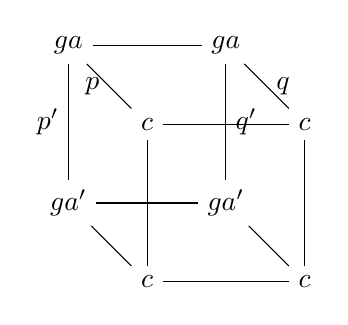
\begin{tikzpicture}
        \node (1) at (0,2) {\( ga \)};
        \node (2) at (2,2) {\( ga\)};
        \node (3) at (1,1) {\( c \)};
        \node (4) at (3,1) {\( c \)};
        \node (5) at (0,0) {\( ga' \)};
        \node (6) at (2,0) {\( ga' \)};
        \node (7) at (1,-1) {\( c \)};
        \node (8) at (3,-1) {\( c \)};
        \draw [-] (1) to node [] {} (2);
        \draw [-] (3) to node [] {} (4);
        \draw [-] (5) to node [] {} (6);
        \draw [-] (7) to node [] {} (8);
        \draw [-] (1) to node [left] {\( p \)} (3);
        \draw [-] (2) to node [right] {\( q \)} (4);
        \draw [-] (5) to node [] {} (7);
        \draw [-] (6) to node [] {} (8);
        \draw [-] (1) to node [left] {\( p' \)} (5);
        \draw [-] (2) to node [right] {\( q' \)} (6);
        \draw [-] (3) to node [] {} (7);
        \draw [-] (4) to node [] {} (8); 
      \end{tikzpicture}
    \]
    commutes and is filled because \( \C \) is a set. Therefore
    %
    \(
         ( p,q ) = ( p',q' ) 
    \)
    % 
%
\end{proof}

We now construct a point
\[
  \code ( \inr c , \ap_{\glue} a ) \tin
  \code ( \inr c , \inl fa ) =
  \code ( \inr c , \inl ga ).
\]
Because both sides of the equality are propositions, a unique
definition for \( \code ( \inr c , \ap_{\glue} a ) \) exists if we
construct an equivalnce.

\begin{lemma} \label{thm:code-cfa-isEquiv-code-cga}
%
  The functions
  \[
    \code ( \inr c , \inl fa ) \to \code ( \inr c , \inr ga ), \:
    ( p,q ) \mapsto p
  \]
  and
  \[
    \code ( \inr c , \inr ga ) \to \code ( \inr c , \inl fa ), \:
    r \mapsto ( r , \refl_{\inl fa} )
  \]
  form an equivalence. 
%
\end{lemma}
\begin{proof}
%
  First, let us show these actually are functions.
  
  Let
  \(
      ( p,q ) \tin \code ( \inr c , \inl fa ).
  \)
  Since \( f \) is injective, we have that
  \(
      a =_\A a' .
  \)
  Beta-reducing \( ga' \) to \( ga \), gives us that
  \(
      p \tin \code ( \inr c , \inr ga ).
  \)
  This provides the first
  function.

  Given
  \(
      r \tin \code ( \inr c , \inr ga ),
  \)
  %
  \( r \) is equal to a
  point in
  \(
      c =_\C ga.
  \)
  This provides a point
  %
  \(
      ( r , \refl_{fa} ) \tin \code ( \inr c , \inl fa ).
  \)
  % 
  This gives the second function.

  The functions form an equivalence Because both
  \( \code ( \inr c , \inl fa ) \) and
  \( \code ( \inr c , \inr ga ) \) are propositions.
\end{proof}

% ~~~~~~~~~~~~~~~~~~~~~~~~~~~~~~

The next stage in proving Theorem \ref{thm:pushout-is-set} is showing
that
%
\(
    \inl b =_{\BAC} x 
\)
% 
and
%
\(
\inr c =_{\BAC} x
\)
% 
are mere propositions for any \( x \).  To do so, we construct
equivalences between, respectively,
%
\(
    \code ( \inl b , x )
\)
% 
and
%
\(
    \code ( \inr c , x )
\)
% 
which we know are mere propositions. Specifically, we define maps
%
\begin{align*}
  \encode ( \inl b ) \from & \prod\limits_{x \tin \BAC}
    ( \inl b =_{\BAC} x ) \to \code ( \inl b , x ) \\
  \encode ( \inr c ) \from & \prod\limits_{x \tin \BAC}
    ( \inr c =_{\BAC} x ) \to \code ( \inr c , x ) \\
  \decode ( \inl b ) \from & \prod\limits_{x \tin \BAC}
    \code ( \inl b , x ) \to ( \inl b =_{\BAC} x ) \\
  \decode ( \inr c ) \from & \prod\limits_{x \tin \BAC}
    \code ( \inr c , x ) \to ( \inr c =_{\BAC} x ) \\
\end{align*}
%
with corresponding \( \encode \) and \( \decode \) pairs forming
mutual equivalences.

% ~~~~~~~~~~~~~~~~~~~~~~~~
% ~~~~~~~~~~~~~~~~~~~~~~~~

\subsection{Defining \( \encode \)}
\label{sec:define-encode}

We define \( \encode ( \inl b ) \) and \( \encode ( \inr
c ) \) by inducting on \( x \tin \BAC \). In doing so, we make use of
path induction. 

Define 
\[
  \encode ( \inl (b) ) \from
  \prod\limits{ x \tin \BAC } ( \inl (b) =_{\BAC} x ) \to
  \code (\inl(b) , x)
\] 
by the assignment
%
\(
    \refl_{\inl b} \mapsto \refl_{\inl' b}.
\)
% 
Recall, \( \inl \) corresponds to the pushout map into \( \BAC \)
and \( \inl' \) to the pushout map into
\( \code ( \inl b , \inl b' ) \).

Define 
\[
  \encode ( \inr c ) \from
  ( \inr c =_{\BAC} x ) \to
  \code ( \inr c , x)
\] 
by the assignemnt
%
\(
    \refl_{ \inr c} \mapsto \refl_c.
\)
% 
Note, we use that
%
\(
    \code ( \inr c , \inr c )
\)
% 
is equivalent to \( c =_\C c \) as shown in Lemma
\ref{sec:code-cc-isProp}.

Define
\[
  \ap_{ \encode ( \inl b ) } \tin
  ( ( b =_{\BAC} fa ) \to \code ( \inl b , \inl fa ) ) =
  ( ( b =_{\BAC} ga ) \to \code ( \inl b , \inr ga ) )
\]
%
to be the diagram
%
\[
  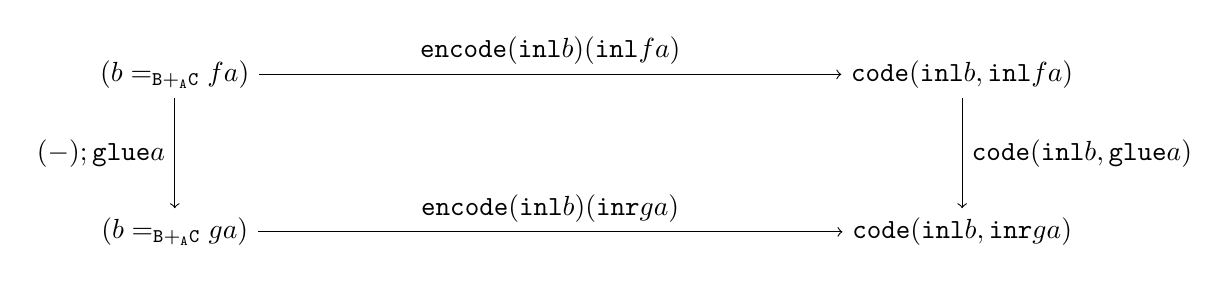
\begin{tikzpicture}
    \node (1) at (-5,1) {\( ( b =_{\BAC} fa ) \)};
    \node (2) at (-5,-1) {\( ( b =_{\BAC} ga ) \)};
    \node (3) at (5,1) {\( \code ( \inl b , \inl fa ) \)};
    \node (4) at (5,-1) {\( \code ( \inl b , \inr ga ) \)};
    \draw [->] (1) to node [left]
      {\( (-) ; \glue a \)} (2);
    \draw [->] (1) to node [above]
      {\( \encode ( \inl b ) ( \inl fa ) \)} (3);
    \draw [->] (2) to node [above]
      {\( \encode ( \inl b ) ( \inr ga ) \)} (4);
    \draw [->] (3) to node [right]
      {\( \code ( \inl b , \glue a ) \)} (4); 
  \end{tikzpicture}
\]
%
which commutes because \( \code ( \inl b , ga ) \) is a mere proposition.
\par

Define
%
\[
  \ap_{ \encode ( \inr c ) } \tin
  ( ( c =_{\BAC} fa ) \to \code ( \inr c , \inl fa ) ) =
  ( ( c =_{\BAC} ga ) \to \code ( \inr c , \inr ga ) )
\]
%
to be the diagram
%
\[
  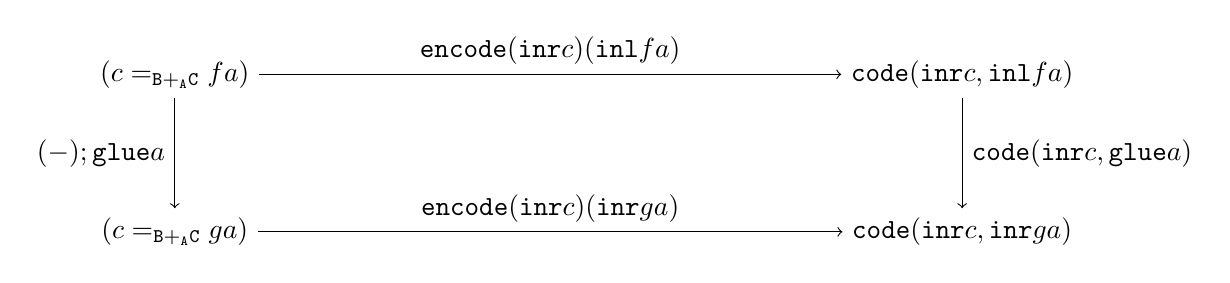
\begin{tikzpicture}
    \node (1) at (-5,1) {\( ( c =_{\BAC} fa ) \)};
    \node (2) at (-5,-1) {\( ( c =_{\BAC} ga ) \)};
    \node (3) at (5,1) {\( \code ( \inr c , \inl fa ) \)};
    \node (4) at (5,-1) {\( \code ( \inr c , \inr ga ) \)};
    \draw [->] (1) to node [left]
      {\( (-) ; \glue a \)} (2);
    \draw [->] (1) to node [above]
      {\( \encode ( \inr c ) ( \inl fa ) \)} (3);
    \draw [->] (2) to node [above]
      {\( \encode ( \inr c ) ( \inr ga ) \)} (4);
    \draw [->] (3) to node [right]
      {\( \code ( \inr c , \glue a ) \)} (4); 
  \end{tikzpicture}
\]
%
which commutes because \( \code ( \inr c , ga ) \) is a mere proposition.
\par

% ~~~~~~~~~~~~~~~~~~~~
% ~~~~~~~~~~~~~~~~~~~~

\subsection{Defining \( \decode \)}
\label{sec:define-decode}

To define the map
%
\begin{equation} \label{eq:decode-b-blank}
%
  \decode ( \inl b ) \from
  \prod\limits_{x \tin \BAC} \code ( \inl b , x ) \to
  ( \inl b =_{\BAC} x )
%
\end{equation}
%
we use induction on \( x \tin \BAC \) which, in practice, means that
we need two function types
%
\begin{itemize}
\item
  \(
    \decode ( \inl b ) ( \inl b' ) \from
    \code (\inl b , \inl b') \to
    ( \inl b =_{\BAC} \inl b' )
  \)
\item
  \(
    \decode ( \inl b ) ( \inl c ) \from
    \code ( \inl b , \inr c ) \to
    ( \inl b =_{\BAC} \inr c
  \) 
\end{itemize}
%
and a witness
%
\begin{align*}
  \ap_{\decode ( \inl b )} (\glue a) &
  \tin
  ( \code ( \inl b , \inl fa ) \to ( \inl b =_{\BAC} \inl fa ) \\
  & =
  ( \code ( \inl b , \inl ga ) \to ( \inl b =_{\BAC} \inl ga )
\end{align*}

% ~~~~~~~~~~~~~~~~~~

Define
\[
  \decode ( \inl b ) \from
  \code ( \inl b , \inl b' ) \to
  ( \inl b =_{\BAC} \inl b' )
\]
by inducting on
%
\(
    \code ( \inl b , \inl b' )
\)
% 
This requires three values.
%
\begin{itemize}
\item
  Let
  \(
    \decode ( \inl b) (\inl' p) \tin ( b =_{\BAC} b' ),
  \)
  where
  \(
    p \tin b =_{\B} b',
  \)
  be
  \(
    \ap_{\inl} (p);
  \)
\item
  Let
  \(
    \decode (\inl b ) ( \inr' (q,r,s) ) \tin ( b ={\BAC} b' ),
  \)
  where
  \(
    (q,r,s) \tin
    \sum\limits_{a,a' \tin \A}
    ( b =_\B fa ) \times (b' =_\B fa' ) \times ( ga =_\C ga' ),
  \)  
  be
  \(
    ap_{\inl} q ; \glue a ; \ap_{\inr} s ; \glue^{-1} a' ; r^{-1}
  \)
  and
\item
  The path
  \begin{align*}
    \ap_{\decode ( \inl b )} ( \glue (t,u,v) )
    & \tin ( \decode ( \inl b )
      ( \inl' ( \alpha (t,u,v) ) ) =_{\inl b =_{\BAC} \inl b'} \\
    & \decode ( \inl b ) ( \inr' ( \beta (t,u,v) ) ),
  \end{align*}
  where
  \(
    (t,u,v) \tin
    ( b =_\B fa ) \times ( b' =_\B fa' ) \times ( b =_\B b' ),
  \)
  is trivial because
  \(
    \code ( \inl b , \inl b' )
  \)
  is a mere set.
\end{itemize}

% ~~~~~~~~~~~~~~~~~~ 

To define
\[
  \decode ( \inl b ) \from
  \code ( \inl b , \inr c ) \to
  ( \inl b =_{\BAC} \inr c ),
\]
recall that
\[
  \code ( \inl b , \inr c ) =
  \sum\limits_{a \tin \A} (b =_{\B} fa) \times (c =_{\C} ga)
\]
Define
\[
  \decode ( \inl b ) ( p , q ) \bydef
  \inl p ; \glue a ; \inr q
\]

% ~~~~~~~~~~~~~~~~~~ 

Right now, we define
%
\begin{align*}
  \ap_{\decode ( \inl b ) } (\glue a) & \tin
  ( \code ( \inl b , \inl fa ) \to ( \inl b =_{\BAC} \inl fa ) \\
  & =
  ( \code ( \inl b , \inl ga ) \to ( \inl b =_{\BAC} \inl ga )
\end{align*}
%
To define this is to construct a commuting square
\[
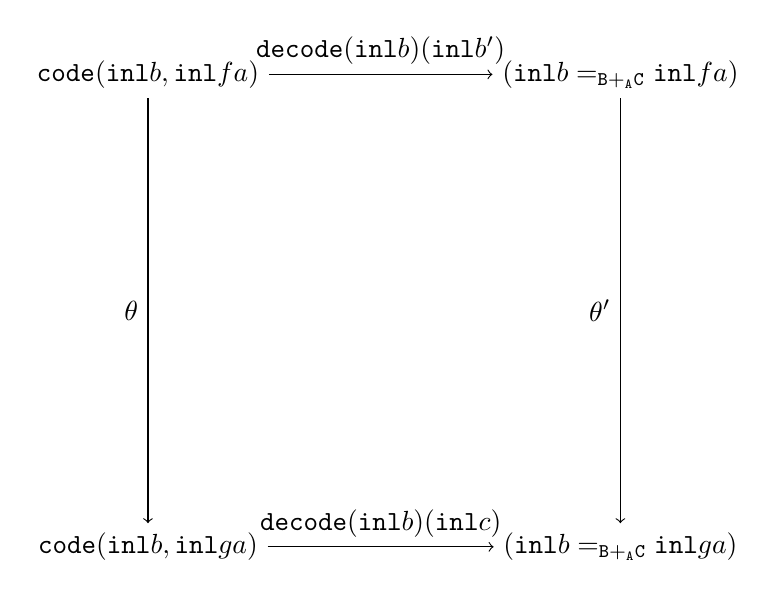
\begin{tikzpicture}
  \node (1) at (-3,3)
    {\( \code ( \inl b , \inl fa ) \)};
  \node (2) at (-3,-3)
    {\( \code ( \inl b , \inl ga ) \)};
  \node (3) at (3,3)
    {\( ( \inl b =_{\BAC} \inl fa ) \)};
  \node (4) at (3,-3)
    {\( ( \inl b =_{\BAC} \inl ga ) \)};
  \draw [->] (1) to node [left]
    {\( \theta \)} (2);
  \draw [->] (1) to node [above]
    {\( \decode (\inl b )(\inl b') \)} (3);
  \draw [->] (3) to node [left]
    {\( \theta' \)} (4);
  \draw [->] (2) to node [above]
    {\( \decode (\inl b )(\inl c) \)} (4);
\end{tikzpicture}
\]
We have already defined the two \( \decode \) maps. The map \( \theta'
\) is post-composition by \( \glue a \). The map \( \theta \) requires
induction to define because we are mapping out of a pushout.
Therefore, we need the following three values to define \( \theta \):
\begin{itemize}
\item
  \(
    \theta (\inl' p)
  \)
  for
  \(
    p \tin b =_\B fa
  \)
\item
  \(
    \theta ( \inr' (q,r,s) )
  \)
  for
  \(
    (q,r,s) \tin
      \sum\limits_{a',a'' \tin \A}
      (b=_\B fa') \times (fa =_B fa'') \times (ga' =_C ga'')
  \) 
\item
  \(
    \ap_{ \theta } ( \glue (t,u,v) ) \tin
      \theta ( \inl' (\alpha (t,u,v) ) ) =
      \theta ( \inr' ( \beta (t,u,v) ) )
  \).
\end{itemize}

A quick remark on notation: since \( f \) is monic and \( \B \) is a
set, we can pull back any path of form \( r \tin fa =_\B fa'\) to a
determined path
\(
  \hat{r} \tin a =_\A a'.
\)

Define
\(
  \theta (\inl' p)
\)
for
\(
  p \tin b=_\B fa
\)
to be
\(
  ( p , \refl_{ga} ).
\)
Define
\(
  \theta ( q,r,s )
\)
to be
\(
  ( q , \ap_g ( \hat{r} ) ; s^{-1} ).
\)

Now we know that
\(
  \ap_{ \theta } ( \glue ( t,u,v ) )
\)
is a path from
\(
  \theta ( \inl' ( v ) ) = ( v , \refl_{ga} )
\)
to
\(
  \theta ( \inr' ( \beta ( t,u,v ) ) )
\)
But that can be reduced:
%
\begin{align*}
  \theta ( \inr' ( t,u,\ap_{g}(\hat{v}) ) )
  & = ( t, \ap_g ( \hat{u} ); \ap_g ( \hat{v} )^{-1} ) \\
  & = ( t, \ap_g ( \hat{u} ; \hat{v}^{-1}) ).
\end{align*}
% 
With this in mind, we define
\(
  \ap_{\theta} ( \glue ( t,u,v ) )
\)
to be post-composition by
\[
  ( \ap_f ( \hat{u};\hat{v}^{-1} ) , \ap_g ( \hat{u};\hat{v}^{-1} ) ).
\]

Now we need to check that the diagram commutes.  Since
\(
  \code ( \inl b , \inl fa )
\)
is a set, it suffices to check that
\[
  \theta' ( \decode (\inl b ) ( \inl fa ) ( x ) )
    =_{ \inl b =_{\BAC} \inr ga }
    \decode ( \inl b )(\inr ga) ( \theta ( x ) )
\]
where
\(
  x \tin \code ( \inl b, \inl fa )
\)
takes values
%
\begin{itemize}
\item
  \(
    \inl' p
  \)
  for
  \(
    p \tin b=_\B fa,
  \)
  and
\item
  \(
    \inr' ( q,r,s )
  \)
  for
  \(
    ( q,r,s ) \tin
      \sum\limits_{a',a'' \tin \A}
      (b=_\B fa') \times ( fa =_\B fa'' )\times ( ga'=_\C ga'' ).
  \)
\end{itemize}
%
We also need to check that
\[
  \ap_{ \theta' ; \decode ( \inl b ) ( \inl fa ) )} ( \glue ( t,u,v ) ) 
    =_{ \inl b =_{\BAC} \inr ga }
    \ap_{ \decode ( \inl b )(\inr ga) ; \theta } ( \glue ( t,u,v ) ) 
\]

Set
\(
  x \bydef \inl' p.
\)
Then
%
\begin{align*}
  \theta' ( \decode ( \inl b ) ( \inl fa ) ( \inl' p ) )
  & = \theta' ( ( \ap_{\inl'} p ) ) \\
  & = \ap_{\inl'} p ; \glue a
\end{align*}
%
Also,
%
\begin{align*}
  \decode ( \inl b ) ( \inr ga ) ( \theta ( \inl' p ) )
  & = \decode ( \inl b ) ( \inr ga ) ( ( p,\refl_{ga} ) ) \\
  & = \ap_{\inl'} p ; \glue a ; \ap_{\inr'} \refl_{ga} \\
  & = \ap_{\inl'} p ; \glue a ; \refl_{\inr' ga} \\
  & = \ap_{\inl'} p ; \glue a
\end{align*}
%
Therefore, the square commutes on \( \inl' p \)

Set
\(
  x \coloneqq \inr' ( q,r,s ).
\)
Then
\begin{align*}
  \theta' ( \decode ( \inl b ) ( \inl fa ) ( \inr' ( q,r,s ) ) )
  & = \theta' ( \ap_{\inl} q ; \glue a' ; \ap_{\inr} s ; \glue a'' ;
    \ap_{\inl} r^{-1} ) \\
  & =  \ap_{\inl} q ; \glue a' ; \ap_{\inr} s ; \glue^{-1} a'' ;
    \ap_{\inl} r^{-1} ; \glue a \\
   & =  \ap_{\inl} q ; \glue a' ; \ap_{\inr} s ; \glue^{-1} a'' ;
    \ap_{\inl} \ap_f \hat{r}^{-1} ; \glue a \\
\end{align*}
%
Also,
%
\begin{align*}
  \decode ( \inl b ) ( \inr ga ) ( \theta ( \inr' ( q,r,s ) ) )
  & = \decode ( \inl b )( \inr ga )( q , \ap_g ( \hat{r} ; s^{-1}
    ) ) \\
  & = \ap_{\inl} q ; \glue a' ; ( \ap_{\inr} ( \ap_g \hat{r} ; s^{-1} )^{-1} ) \\
  & = \ap_{\inl} q ; \glue a' ; \ap_{\inr} ( \ap_g ( \hat{r} ) ; ( \ap_g
    (s^{-1}) )^{-1} ) \\
  & = \ap_{\inl} q ; \glue a' ; \ap_{\inr} (s^{-1})^{-1} ;  \ap_g ( \hat{r} )^{-1} \\
  & = \ap_{\inl} q ; \glue a' ; \ap_{\inr} (s^{-1})^{-1} ;  \ap_g ( \hat{r} )^{-1} \\
  & = \ap_{\inl} q ; \glue a' ; \ap_{\inr} s ;  \ap_g ( \hat{r} )^{-1} \\
\end{align*}
%
We just need to check that
\[
  \ap_g ( \hat{r} )\inv =
  \glue\inv a'' ; \ap_{ \inl } \ap_f \hat{r}\inv ; \glue a
\]
But this follows from the continuity of \( \glue \), that is, it
preserves paths. Therefore, the square commutes on
\(
  \inr' ( q,r,s ).
\)

It remains to check that
\[
  \ap_{\theta' ; \decode (\inl b ) ( \inl fa ) )} ( \glue ( t,u,v ) ) 
  =_{ \inl b =_{\BAC} \inr ga }
  \ap_{ \decode ( \inl b )(\inr ga) ; \theta } ( \glue ( t,u,v ) ) 
\]
for
\(
  ( t,u,v ) \tin
  \sum\limits_{a',a''\tin \A}
  ( b =_\B fa' ) \times ( fa =_\B fa'' ) \times ( b =_{\B} fa ).
\)
Here, we make some reductions.
%
\begin{itemize}
\item
  Because \( f \) is monic, we get that
  \(
    fa =_\B fa''
  \)
  reduces to
  \(
    fa =_\B fa.
  \)
  Since \( \B \) is a set, we can take
  \(
    u = \refl_{fa}.
  \)
\item
  The type
  \(
    b =_\B fa'
  \)
  reduces to
  \(
    fa =_\B fa
  \)
  because \( \B \)
  is monic, so
  \(
    t = \refl_{fa}.
  \).
\item
  The type
  \(
    b =_\B fa
  \)
  reduces to
  \(
    fa =_\B fa
  \)
  because \( \B \) is monic, so
  \(
    v = \refl_{fa}.
  \)
\end{itemize}
%
Without loss of generality, we can take
\(
  ( t,u,v ) = ( \refl_{fa},\refl_{fa},\refl_{fa} ).
\)
Therefore, it suffices to check that 
\begin{align*}
%
   & \ap_{\theta' ; \decode (\inl b ) ( \inl fa ) )}
   ( \glue ( \refl_{fa},\refl_{fa},\refl_{fa} ) ) \\
        & =_{ \inl b =_{\BAC} \inr ga }
        \ap_{ \decode ( \inl b )( \inr ga ) ; \theta }
        ( \glue  ( \refl_{fa},\refl_{fa},\refl_{fa} ) ). 
% 
\end{align*}
  
But because the square commutes on points as shown above, the two
paths on the left and right of the above equation are certainly
parallel.  Then functorality gives us that \( \refl_{fa} \) is
preserved. Hence the square commutes.

% ~~~~~~~~~~~~~~~~~~~

To define the map
\[
  \decode ( \inr c ) \from
  \prod\limits_{x \tin \BAC}
  \code ( \inr c , x ) \to \inr ( c =_{\BAC} x )
\]
we use induction on \( \BAC \) which, in practice, means that we
require the two function types
%
\begin{itemize}
\item
  \(
    \decode ( \inr c ) ( \inl b ) \from
      \code (\inr c , \inl b) \to
      ( \inr c =_{\BAC} \inl b )
  \)
\item
  \(
    \decode ( \inr c ) ( \inr c' ) \from
      \code ( \inr c , \inr c' ) \to
      ( \inr c =_{\BAC} \inr c' )
  \) 
\end{itemize}
%
and a witness
%
\begin{align*}
  \ap_{\decode ( \inr c ) } (\glue a) & \tin
  ( \code ( \inr c , \inl fa ) \to ( \inr c =_{\BAC} \inl fa ) \\
  & = ( \code ( \inr c , \inl ga ) \to ( \inr c =_{\BAC} \inl ga )
\end{align*}

% ~~~~~~~~~~~~~~~~~~~~``

First, let us define the map
\[
  \decode ( \inr c ) ( \inl b ) \from
    \code ( \inr c , \inl b ) \to
    ( \inr c =_{\BAC} \inl b ).
\]
Recall that
\(
  \code ( \inr c , \inl b ) \coloneqq
    \sum\limits_{a \tin \A}
    ( c =_{\C} ga ) \times ( b =_{\B} fa ).
\)
Thus for any \( ( p,q ) \) in
\(
  \code ( \inr c , \inl b ),
\)
we define a path
\(
  \decode ( \inr c ) ( \inl b ) ( p,q )
\)
in \( \BAC \) from \( \inr c \) to  \( \inl b \). Take this path to be
\(
  \inr p ; \glue^{-1}  a ; \inl q^{-1}.
\)

% ~~~~~~~~~~~~~~~~~

Next, we define
\[
  \decode ( \inr c ) ( \inr c' ) \from
  \code ( \inr c , \inr c' ) \to
  ( \inr c =_{\BAC} \inr c' ).
\]
Recall that
\[
  \code ( \inr c , \inr c' ) \bydef
  \sum\limits_{a \tin \A}
  ( c =_{\C} ga ) \times ( c' =_{\C} ga' ) \times ( fa =_{\B} fa' ). 
\]
Thus for any \( ( p,q,r ) \) in
\(
  \code ( \inr c , \inr c' ),
\)
we define a path
\(
  \decode ( \inr c ) ( \inr c' ) ( p,q,r )
\)
in \( \BAC \) from \( \inr c \) to \( \inr c' \). Take this path to be
\(
  \inr p ; \glue\inv a ; \inl r \glue a' ; \inr q\inv.
\)

% ~~~~~~~~~~~~~~~~~~

Finally, we define a path
%
\begin{align*}
  \ap_{\decode ( \inr c )} (\glue a) & \tin
  ( \code ( \inr c , \inl fa ) \to ( \inr c =_{\BAC} \inl fa ) \\
  & =  ( \code ( \inr c , \inl ga ) \to ( \inr c =_{\BAC} \inl ga ).
\end{align*}
%
Replacing the two \( \code \) expressions with their definitions, this
path is constructed as a commuting square
\[
  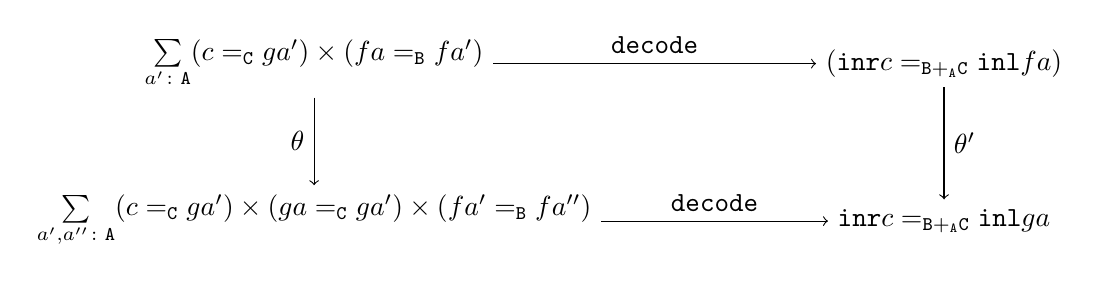
\begin{tikzpicture}
    \node (1) at (-4,1)
      { \(
        \sum\limits_{a' \tin \A}
        ( c =_{\C} ga' ) \times ( fa =_{\B} fa' )
      \) }; 
    \node (2) at (-4,-1)
      { \(
        \sum\limits_{a',a'' \tin \A}
        ( c =_{\C} ga' ) \times ( ga =_{\C} ga' ) \times
        ( fa' =_{\B} fa'' )
      \) };
    \node (3) at (4,1)
      { \(
        ( \inr c =_{\BAC} \inl fa )
      \) };
    \node (4) at (4,-1)
      { \(
        \inr c =_{\BAC} \inl ga
      \) };
    \draw [->] (1) to node [left] {\( \theta \)} (2);
    \draw [->] (1) to node [above] {\( \decode \)} (3);
    \draw [->] (2) to node [above] {\( \decode \)} (4);
    \draw [->] (3) to node [right] {\( \theta' \)} (4); 
  \end{tikzpicture}
\]
The easier map to define is \( \theta' \) which  concatenates
with \( \glue a \).  Then \( \theta \) is given by
\(
  ( p,q ) \mapsto ( p, \refl_{ga} , q ).
\)
Now we check whether the square commutes. We have
%
\begin{align*}
  \theta' ( \decode ( \inr c , - ) ( \inl fa ) ( p,q ) )
  & = \theta' ( \inr p ; \glue^{-1} a' ; \inl q^{-1}  ) \\
  & = \inr p ; \glue^{-1} a' ; \inl q^{-1} ; \glue a. \\
\end{align*}
%
We also have that
%
\begin{align*}
  \decode ( \inr c , - ) ( \inl ga ) ( \theta ( p,q ) )
  & = \decode ( \inr c , - ) ( \inl ga ) ( p,\refl_{ga},q ) \\
  & =  \inr p ; \glue\inv a' ; \inl q\inv ; \glue a ; \inr \refl_{ga} \\
  & =  \inr p ; \glue\inv a' ; \inl q\inv ; \glue a  \\
\end{align*}
%
Hence the square commutes.

% ~~~~~~~~~~~~~~~~~~~~~~~~
% ~~~~~~~~~~~~~~~~~~~~~~~~
% ~~~~~~~~~~~~~~~~~~~~~~~~
% ~~~~~~~~~~~~~~~~~~~~~~~~

\subsection{Composing encode and decode}

Consider the composite
\[
  \encode ; \decode
  \from
  \prod\limits_{x,y \tin \BAC} x =_{\BAC} y
  x =_{\BAC} y
\]
To show that this map is the identity up to homotopy, we compute both
%
\begin{itemize}
\item
  \(
    \encode ; \decode ( \inl b ) \from
      \prod\limits_{x \tin \BAC}
      ( \inl b =_{\BAC} x ) \to ( \inl b =_{\BAC} x ),
   \)
   and
\item
  \(
    \encode ; \decode ( \inr c  ) \from
      \prod\limits_{x \tin \BAC}
      \inr c =_{\BAC} x \to ( \inr c =_{\BAC} x ).
  \)
\end{itemize}
%
But computing these values actually requires the computation of the
following four maps:
\begin{itemize}
\item
  \(
    \encode ; \decode ( \inl b )(\inl b') \from
      \code ( \inl b , \inl b' ) \to
      ( \inl b =_{\BAC} \inl b' ).
  \)
  By path induction, it suffices to check \( \refl_{\inl b} \):
  \begin{align*}
    \encode ; \decode ( \inl b )(\inl b') ( \refl_{\inl b} ) & =
    \encode ( \ap_{\inl'} \refl_{\inl b} ) \\ & =
    \encode (\refl_{\inl' b} ) \\ & =
    \ap_{\inl} \refl_{\inl' b} \\ & =
    \refl_{\inl b}.
  \end{align*}
  So this one checks out.
\item
  \(
    \encode ; \decode ( \inl b ) (\inr c) \from
      \code ( \inl b , \inr c ) \to
      ( \inl b =_{\BAC} \inl c ).
  \)
  \edit{glue(a) *is* the only thing to check here, right?}
  This is only non-trivial when
  \(
    b =_\B fa
  \)
  and
  \(
    c =_\C ga.
  \)
  Hence
  \[
    \encode ; \decode ( \inl b ) ( \inr c ) ( \glue a ) =
    \decode ( \inl b ) ( \inr c ) ( \refl_{fa} , \refl_{ga} ) =
    \ap_{\inr} \refl_{ga} ; \glue a ; \ap_{\inl} \refl_{fa} =
    \glue a.
  \]
  This one checks out too.
\item
  \(
    \encode ; \decode ( \inr c , - )(\inl b) \from
    \code ( \inr c , \inl b ) \to ( \inr c =_{\BAC} \inl b ).
  \)
  This is symmetric to the above case, so checks out. 
\item
  \(
  \encode ; \decode ( \inr c , - )(\inr c') \from
  \code ( \inr c, \inr c' ) \to
  ( \inr c =_{\BAC} \inr c' )
  \)
  is, by path induction, 
  \[
    \encode ; \decode ( \inr c , - )(\inr c') ( \refl_{\inr c} ) =
    \decode ( \inr c , - )(\inr c') ( \refl_c ) =
    \ap_{\inr} \refl_c =
    \refl_{\inr c}
  \]  
\end{itemize}

And so, we have proved that \( \decode \) is a section for \( \encode
\). The opposite direction remains.

% ~~~~~~~~~~~~~~~~~~

Now, we look at the composite
\[
  \decode ; \encode \from
  \prod\limits_{x,y \tin \BAC} \code ( x,y ) \to
  \code ( x,y )
\]
We can compute this composite by computing the values
%
\begin{itemize}
\item
  \(
    \decode ; \encode (\inl b ) ( \inl b' ) \from
    \code ( \inl b , \inl b' ) \to
    \code ( \inl b , \inl b' ),
  \)
\item
  \(
    \decode ; \encode (\inl b ) ( \inr c ) \from
    \code ( \inl b , \inr c ) \to
    \code ( \inl b , \inr c ),
  \)
\item
  \(
    \decode ; \encode (\inr c ) ( \inl b ) \from
    \code ( \inr c , \inl b ) \to
    \code ( \inr c , \inl b ),
    \)
  and  
\item
  \(
    \decode ; \encode (\inr c ) ( \inr c' ) \from
    \code ( \inr c , \inr c' ) \to
    \code ( \inr c , \inr c' )
  \)
\end{itemize}
%
But these maps are all identity since \( \code (x,y) \) is a
proposition for \( x , y \tin \BAC \).   
\par

% ~~~~~~~~~~~~~~~~~~

We now know that
% 
\(
    \encode
\)
%
and
%
\(
    \decode
\)
% 
are mutual inverses. Therefore,
% 
\(
    \inl b =_{ \BAC  } x
\)
% 
and
%
\(
    \inr c =_{ \BAC } x
\)
% 
are mere propositions for any
%
\(
    x \tin \BAC.
\)
% 
As discussed above, the embedding
% 
\(
    \P \hookrightarrow \Q
\)
%
is actually an equivlance. Theorem \ref{thm:pushout-is-set} follows.

% =======================================
\section{Cohomology in $ \zmodtwo $}
\label{sec:cohomology--zz2zz}
% =======================================

\textbf{Strategy:}
Use that $ \pi_{n+m} ( K(G,n) \wedge K(H,m) ) = G \otimes H
$ to show, for $ R \coloneqq \zmodtwo $, that $ || K(R,n)
\wedge K(R,m) ||_{n+m} = K( R \otimes R, n+m ) $. Then we' will
lift the ring multiplication $ R \otimes R \to R $ to a cup
product on cohomology with $ R $-coefficients.

First, we show that
$ || K(R,n) \wedge K(R,m) ||_{n+m} = K( R \otimes R, n+m )
$. We use the fact that $K (R \otimes R, n+m )$ is the unique up to homotopy space
having the property that
\[
  \pi_k (K(R \otimes R, n+m )) =
  \begin{cases}
    0, & k \neq n+m \\
    R \otimes R, & k= n+m \\
  \end{cases}
\]
Thus by showing that $ || K(R,n) \wedge K(R,m) ||_{n+m} $
has the property, we have the desired
equivalence. First, (see [Strom, Prop 19.60]) we have that
\[
  \pi_{n+m} ( || K(R,n) \wedge K(R,m) ||_{n+m} )
  = R \otimes R.
\]
Second, we have that
\[
  \pi_k ( || K(R,n) \wedge K(R,m) ||_{n+m} )
  = 0
\]
for $ k > n+m $ because $ || K(R,n) \wedge K(R,m) ||_{n+m} $
is an $ ( n+m ) $-type. Third, we have that 
\[
  \pi_k (|| K(R,n) \wedge K(R,m) ||_{n+m} ) = 0
\]
for $ k \leq n+m-1 $ because
$ || K(R,n) \wedge K(R,m) ||_{n+m} $ is
$ ( n+m-1 ) $-connected, which follows from $ K( R,k ) $ being
$ ( k-1 ) $-connected, as seen in Guillame's
thesis Prop 4.3.1. From these three facts, we conclude that
\[
  \pi_k (|| K(R,n) \wedge K(R,m) ||_{n+m}) =
  \begin{cases}
    0, & k \neq n+m \\
    R \otimes R, & k= n+m \\
  \end{cases}
\]
and, in particular, we get that
\[
  || K(R,n) \wedge K(R,m) ||_{n+m} \simeq
  K (R \otimes R, n+m ).
\]
Evoking the univalence axiom, we get that
\[
  || K(R,n) \wedge K(R,m) ||_{n+m} =
  K (R \otimes R, n+m ).
\]

Now, we construct the ring structure on cohomology. The
strategy is to define structures and property on EM-spaces
then lift those up to cohomology. We begin by defining our
EM-spaces.  Following Licata and Finster's construction of
EM-spaces, we define as follows:
\begin{align*}
  K(\zmodtwo,0) &\coloneqq \zmodtwo \\
  K(\zmodtwo,n) &\coloneqq || \Sigma_{n-1} \rptwo ||_n
\end{align*}
To simplify the notation, we write $ K_n $ for
$ K( \zmodtwo,n) $ when feeling laze.  Addition and subtraction
operations of type $ K_n \times K_n \to K_n $ follow
directly from Guillaume'sthesis Proposition 5.1.4. Let's do
multiplication. From the multiplication
$ \zmodtwo \otimes \zmodtwo \to \zmodtwo $, we get a multiplication
$ K(\zmodtwo \otimes \zmodtwo, n)\to K(\zmodtwo, n) $ by applying the
functor
\[
  K(-,n) \from \mathbf{Ring} \to \mathbf{Ho}(\mathbf{Top_\ast})
\]
But
\[
  || K(R,n) \wedge K(R,m) ||_{n+m} =
  K (R \otimes R, n+m ).
\]
for any ring $ R $ as we showed above, and so we can treat our multiplication as
\[
  \widehat{\mu} \from
  || K(\zmodtwo,n) \wedge K(\zmodtwo,m) ||_{n+m} \to K(\zmodtwo, n+m).
\]
However, we \emph{really} want the domain of multiplication
to be $ K ( \zmodtwo , n) \times K( \zmodtwo, m) $. To get this, we
precompose $ \widehat{\mu} $ by several canonical arrows
resulting in the composite
\[
    K (\zmodtwo , n) \times K(\zmodtwo, m)
      \xrightarrow{\mathtt{proj}}
      K (\zmodtwo , n) \wedge K(\zmodtwo, m)
      \xrightarrow{|-|_{n+m}}
      || K (\zmodtwo , n) \wedge K(\zmodtwo, m) ||_{n+m}
      \xrightarrow{\widehat{\mu}}
      K(\zmodtwo, n+m)
\]
that we call \emph{multiplication} $ \mu $.  This induces
the cup product
\[
  \smile \from H^n(X) \times H^m(X) \to H^{n+m}(X)
\]
on cohomology. Recall that we define the $ n $-th cohomology
with $ \zmodtwo $-coefficients to be
$ H^n (X) \coloneqq || X \to_\ast K_n ||_0 $. This is the
standard definition in homotopy type theory, we do not use
singular cochains, because taking the set up cochains is not
a continuous process. Define
$ \smile ( |\alpha|, |\beta|) ) $, for
$ \alpha \from X \to_\ast K_n $ and
$ \beta ]from X \to K_m $, to be the truncation of the
pairing $ \langle \alpha, \beta \rangle $ followed by $ \mu $:
\[
  \smile ( |\alpha|, |\beta|) ) :
  || X \to K_n \times K_m \to K_{n+m} ||_0.
\]
Thus $ \smile ( |\alpha|, |\beta|) ) $ type-checks. It
remains to show the usual ring properties hold for $ H^n(X)
$.  Distributivity follows directly from Guillaume's
argument in Proposition 5.1.7 which uses only connectivity
hence carries through to our context without issue.  To show
'graded commutativity', it suffices to show standard
commutativity because of the $ \zmodtwo $-coefficients.  






%%%%%%%%%%%%%
% end document
%%%%%%%%%%%%%

\end{document}
